\chapter{Dostosowanie Sirius Web dla systemu BalticLSC}

Z przygotowanego metamodelu języka \CAL{} systemu \BalticLSC{}
opisanego w rozdziale~\ref{chapter:cal-metamodel} do~tej~pory korzystano w
\SiriusDesktop{}, w którym to został on przygotowany. W~tym~rozdziale
zostaną opisane kroki potrzebne do użycia go w \SiriusWeb{}, aby otrzymać
aplikację przeglądarkową umożliwiającą edycję modeli języka \CAL{}.
Zostaną również omówione modyfikacje edytora \SiriusWeb{}, które
zostały wykonane, aby poprawić jego integrację z~systemem \BalticLSC{} oraz
umożliwić realizację walidacji semantycznej modelu.

Obie te rzeczy zostały
wykonane bez dokumentacji technicznej rozwiązania \SiriusWeb{}, bazując na
wielu różnych źródłach wiedzy opisujących części procesu konieczne do
wykonania, oraz na podstawie analizy kodu źródłowego.
Jest to jedno z pierwszych w takim stopniu zmodyfikowanych wykorzystań
technologii \SiriusWeb{} do przygotowania edytora modeli.

\section{Użycie metamodelu języka CAL w Sirius Web}

Chcąc wykorzystać metamodel w formacie \Ecore{} w \SiriusWeb{} należy wskazać
gdzie
on~się~znajduje oraz z jakich klas się składa, aby klasy te mogły zostać
dołączone do pliku \JAR{} serwera, a później odczytane przez moduły
\SiriusWeb{} podczas uruchamiania aplikacji.

Dla \SiriusWeb{} nie istnieje obecnie dokumentacja, co utrudnia jego
wykorzystanie z~własnym metamodelem. W serwisie \GitHub{} istnieje repozytorium
\texttt{sirius-web}~\cite{sirius-web-github} zawierające kod~źródłowy aplikacji
przeglądarkowej
bazującej na \SiriusWeb{}. Jest ona skonfigurowana do~wykorzystywania
metamodelu \emph{Sample Flow}~\cite{flow-network-github}
przygotowanego przez firmę \emph{Obeo Network}. Znajduje się on w innym
repozytorium (\texttt{Flow-Designer}~\cite{flow-network-github}) i jest
zwykłym metamodelem w formacie \Ecore{}.
Należy więc wzorować się na tym przykładowym repozytorium w celu stworzenia
własnego edytora modeli.
W ramach tej pracy magisterskiej stworzono kopię repozytorium
\texttt{sirius-web} i skonfigurowano je, aby wykorzystywało metamodel
języka \CAL{} opisany w~rozdziale~\ref{chapter:cal-metamodel}.

\SiriusWeb{} do zarządzania projektem i wyrażania zależności między
pakietami wykorzystuje narzędzie \emph{Apache Maven}~\cite{maven-homepage}.
Aby wykorzystać klasy metamodelu w formacie \Ecore{} w \SiriusWeb{}
należy do katalogów wygenerowanych przez \SiriusDesktop{} dodać pliki
\POM{} (\texttt{pom.xml}), które zawierają informacje o nazwie projektu i
jego
zależnościach. Wygenerowane na podstawie metamodelu w formacie \Ecore{}
projekty są w formacie projektów \Eclipse{}.
Oznacza to, że ich zależności są zapisane w plikach
\texttt{MANIFEST.MF}, a pozostałe informacje o~projektach znajdują się w
plikach \texttt{build.properties}, \texttt{plugin.properties} oraz
\texttt{plugin.xml}. Te pliki nie są wykrywane domyślnie przez \Maven{},
więc
próba wykorzystania takiego projektu zakończy się błędem. Aby wykorzystać je w
\SiriusWeb{} należy odpowiednio skonfigurować ich pliki
\POM{}~\cite{maven-tycho-tutorial}.

Po pierwsze należy do listy repozytoriów pakietów dodać repozytorium
\Eclipse{} w formacie \texttt{p2}. Jest to format wykorzystywany przez
projekty \Eclipse{}, podczas gdy \Maven{} wykorzystuje repozytoria w
swoim własnym formacie. Fragment pliku \texttt{pom.xml} konfigurujący to
repozytorium znajduje się na listingu~\ref{lst:pom-eclipse-repository}.

\begin{lstlisting}[float,
    floatplacement=ht,
    language=XML,
    caption={Konfiguracja repozytorium \Eclipse{} w \texttt{pom.xml}},
    label={lst:pom-eclipse-repository}]
<repositories>
  <repository>
    <id>eclipse</id>
    <layout>p2</layout>
    <url>http://download.eclipse.org/releases/2021-09</url>
  </repository>
</repositories>
\end{lstlisting}

Kolejno w plikach \texttt{pom.xml} projektów metamodelu w formacie \Ecore{}
należy
zdefiniować, że~są~to~projekty \Eclipse{}, poprzez dodanie elementu
\texttt{packaging} z wartością \texttt{eclipse-plugin}. Zostało
to~zademonstrowane na listingu~\ref{lst:pom-packaging} w linii 9.

\begin{lstlisting}[float,
    floatplacement=hb,
    language=XML,
    caption={Plik \texttt{pom.xml} dla jednego z projektów metamodelu
      w formacie \Ecore{}},
    label={lst:pom-packaging}]
<?xml version="1.0" encoding="UTF-8" ?>
<project
  xmlns="http://maven.apache.org/POM/4.0.0"
  xmlns:xsi="http://www.w3.org/2001/XMLSchema-instance"
  xsi:schemaLocation="http://maven.apache.org/POM/4.0.0 http://maven.apache.org/xsd/maven-4.0.0.xsd"
>
  <modelVersion>4.0.0</modelVersion>
  <artifactId>eu.balticlsc.model.CAL</artifactId>
  <packaging>eclipse-plugin</packaging>

  <parent>
    <groupId>eu.balticlsc.model</groupId>
    <artifactId>model</artifactId>
    <version>0.1.0-SNAPSHOT</version>
  </parent>
</project>
\end{lstlisting}

Następnie w sekcji \texttt{build} pliku \texttt{pom.xml} należy dodać pluginy
\emph{Maven Tycho}~\cite{maven-tycho-homepage}. Jest~to~zestaw rozszerzeń do
\emph{Apache Maven}
pozwalający na wykorzystanie projektów \Eclipse{}. Fragment
wymaganej konfiguracji znajduje się na
listingu~\ref{lst:pom-maven-tycho-plugins}. Ważne jest, aby wskazać konkretną
wersję środowiska uruchomieniowego języka \Java{}. W tym przypadku jest to
Java~11. Jest~to~jedyna wersja oficjalnie obsługiwana przez \SiriusWeb{}.
Inne wersje nie są wspierane.

% TODO: spróbować żeby listingi nie były "na kupie", tylko poprzedzielane tekstem

\begin{lstlisting}[float,
    floatplacement=hb,
    language=XML,
    caption={Konfiguracja rozszerzeń \emph{Maven Tycho} w \texttt{pom.xml}},
    label={lst:pom-maven-tycho-plugins}]
<build>
  <plugins>
    <plugin>
      <groupId>org.eclipse.tycho</groupId>
      <artifactId>tycho-maven-plugin</artifactId>
      <version>2.5.0</version>
      <extensions>true</extensions>
    </plugin>

    <plugin>
      <groupId>org.eclipse.tycho</groupId>
        <artifactId>tycho-packaging-plugin</artifactId>
         <version>2.5.0</version>
         <executions>
          <execution>
            <phase>package</phase>
            <id>package-feature</id>
              <configuration>
                <finalName>${project.artifactId}_${unqualifiedVersion}.${buildQualifier}</finalName>
              </configuration>
        </execution>
      </executions>
    </plugin>

    <plugin>
      <groupId>org.eclipse.tycho</groupId>
      <artifactId>target-platform-configuration</artifactId>
      <version>2.5.0</version>

      <configuration>
        <executionEnvironment>JavaSE-11</executionEnvironment>

        <!-- ... konfiguracja platformy -->
      </configuration>
    </plugin>
  </plugins>
</build>
\end{lstlisting}

Tak przygotowany projekt \Maven{} będzie wykrywał zależności zdefiniowane w
odpowiednich plikach \Eclipse{} i będzie możliwy do wykorzystania jako
zależność w innych projektach \Maven{}. Można to potwierdzić uruchamiając
komendę \lstinline{mvn clean verify}. Model można teraz dodać do pliku
\texttt{pom.xml} aplikacji serwerowej \SiriusWeb{} (projekt
\texttt{sirius-web-sample-application}) dodając odwołania do 3 pakietów:
głównego pakietu modelu, pakietu \texttt{.edit} oraz pakietu \texttt{.design}.
Odwołania te widoczne są na listingu~\ref{lst:pom-metamodel-dependencies}.

\begin{lstlisting}[float,
    floatplacement=hb,
    language=XML,
    caption={Odwołania do pakietów metamodelu w \texttt{pom.xml} aplikacji
    serwerowej \SiriusWeb{}},
    label={lst:pom-metamodel-dependencies}]
<dependency>
  <groupId>eu.balticlsc.model</groupId>
  <artifactId>eu.balticlsc.model.CAL</artifactId>
  <version>0.1.0-SNAPSHOT</version>
</dependency>
<dependency>
  <groupId>eu.balticlsc.model</groupId>
  <artifactId>eu.balticlsc.model.CAL.edit</artifactId>
  <version>0.1.0-SNAPSHOT</version>
</dependency>
<dependency>
  <groupId>eu.balticlsc.model</groupId>
  <artifactId>eu.balticlsc.model.CAL.design</artifactId>
  <version>0.1.0-SNAPSHOT</version>
</dependency>
\end{lstlisting}

Taka konfiguracja zależności między projektami pozwala na wykorzystanie klas
metamodelu w kodzie źródłowym \SiriusWeb{}. Należy teraz w klasie
\texttt{SampleEMFConfiguration} zarejestrować klasy
odpowiedzialne za metamodel: \texttt{EPackage} oraz \texttt{AdapterFactory}.
Fragment kodu realizujący to jest znajduje się na
listingu~\ref{lst:registering-emf-classes}. Później w klasie
\texttt{SampleSiriusConfiguration} należy wskazać ścieżkę do pliku
\texttt{*.odesign} metamodelu znajdującego się w pakiecie \texttt{.design}.
Odpowiedni fragment znajduje się na
listingu~\ref{lst:registering-odesign-path}.

\begin{lstlisting}[float,
    floatplacement=hb,
    language=Java,
    caption={Rejestracja klas przygotowanego metamodelu w klasie
      \texttt{Sample\-EMF\-Configuration}},
    label={lst:registering-emf-classes}]
    @Bean
    public AdapterFactory calAdapterFactory() {
        return new CALItemProviderAdapterFactory();
    }

    @Bean
    public EPackage calEPackage() {
        return CALPackage.eINSTANCE;
    }
\end{lstlisting}

\begin{lstlisting}[float,
    floatplacement=hb,
    language=Java,
    caption={Wskazanie ścieżki do pliku \texttt{*.odesign} w klasie
      \texttt{SampleSiriusConfiguration}},
    label={lst:registering-odesign-path}]
    @Override
    public List<String> getODesignPaths() {
        return List.of("description/CAL.odesign"); //$NON-NLS-1$
    }
\end{lstlisting}

Po tych modyfikacjach w aplikacji \SiriusWeb{} można tworzyć i edytować
modele nowo stworzonego w formacie \Ecore{} metamodelu. Zrzut ekranu z
aplikacji
przeglądarkowej widoczny jest
na~rysunku~\ref{rys:sirius-web-base-metamodel-model}.

% \begin{noindent}
\begin{figure}[!ht]
  \centering

  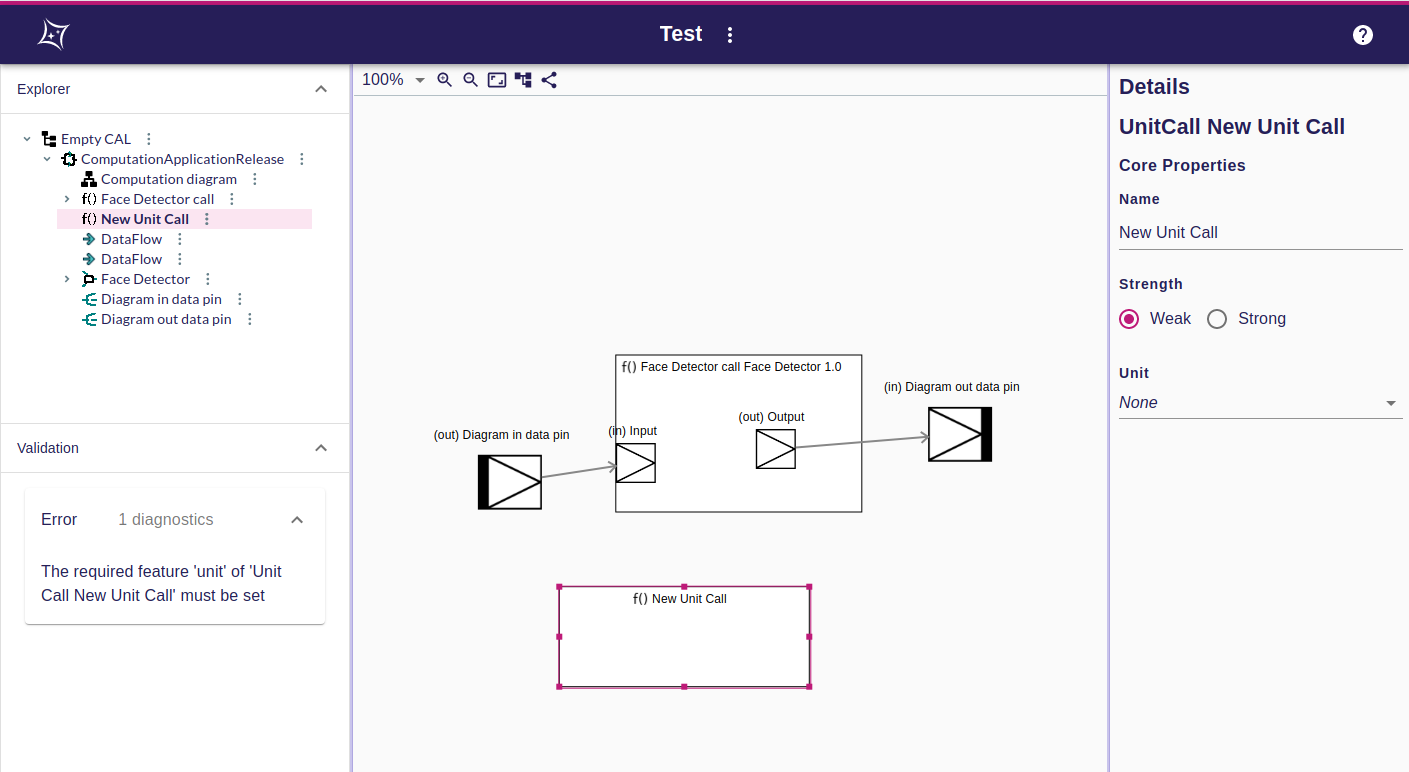
\includegraphics[width=0.95\linewidth]{./images/sirius-web-base-metamodel-model.png}
  \caption{Edycja modelu bazującego na przygotowanym metamodelu języka \CAL{} w
    \SiriusWeb{}}\label{rys:sirius-web-base-metamodel-model}
\end{figure}
% \end{noindent}

W \SiriusWeb{} można zdefiniować szablony modeli, które użytkownik może
wykorzystać chcąc stworzyć nowy model w projekcie. Umożliwia to prostszy
sposób na stworzenie chociażby pustego modelu, ponieważ przycisk tworzenia
modelu
na podstawie szablonu jest bardziej wyeksponowany w interfejsie użytkownika niż
przyciski tworzenia modelu z drzewa elementów projektu po lewej stronie.
Aby dodać nowy szablon należy dodać nowy opis \emph{stereotypu} w metodzie
\texttt{addStereotypeDescriptions} klasy
\texttt{StereotypeDescriptionRegistryConfigurer}. Kod odpowiedzialny za dodanie
nowego pustego szablonu modelu został przedstawiony
na~listingu~\ref{lst:empty-cal-model-template}. Interfejs użytkownika aplikacji
\SiriusWeb{} wyświetlający nowo dodany szablon pustego modelu języka
\CAL{} został przedstawiony na
rysunku~\ref{rys:sirius-web-new-model-template}.

\begin{lstlisting}[float,
    floatplacement=!hb,
    language=Java,
    caption={Dodanie nowego pustego szablonu modelu języka \CAL{}},
    label={lst:empty-cal-model-template}]
    @Override
    public void addStereotypeDescriptions(IStereotypeDescriptionRegistry registry) {
        registry.add(new StereotypeDescription(
          UUID.nameUUIDFromBytes("empty_cal".getBytes()), //$NON-NLS-1$
          "Empty CAL", //$NON-NLS-1$
          this::getEmptyCALContent
        ));
    }

    private String getEmptyCALContent() {
        return this.stereotypeBuilder.getStereotypeBody(
          CALFactory.eINSTANCE.createComputationApplicationRelease()
        );
    }
\end{lstlisting}

% \begin{noindent}
\begin{figure}[!ht]
  \centering

  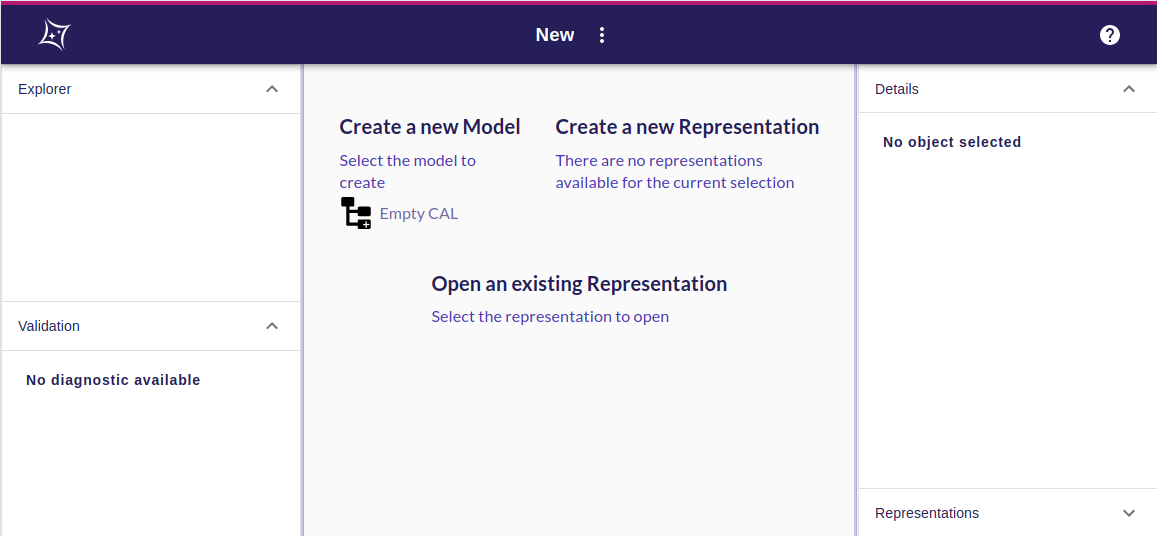
\includegraphics[width=0.95\linewidth]{./images/sirius-web-new-model-template.png}
  \caption{Szablon nowego pustego modelu języka
    \CAL{} w \SiriusWeb{}}\label{rys:sirius-web-new-model-template}
\end{figure}
% \end{noindent}

\subsection{Uruchamianie testów metamodelu za pomocą Maven}

W sekcji~\ref{sec:testy-metamodelu} opisano testy zmodyfikowanego zachowania
metamodelu języka \CAL{} opisanego w formacie \Ecore{}. Były one~uruchamianie w
\SiriusDesktop{}. Z uwagi na fakt, że
wygenerowany projekt z testami jest projektem typu \Eclipse{}, \emph{Apache
	Maven} nie ma możliwości wykonania tych testów podczas standardowego
polecenia wykonania testów \lstinline{mvn test}.

Z pomocą przychodzi tutaj zestaw narzędzi \emph{Maven Tycho} wykorzystany do
połączenia metamodelu w formacie \Ecore{} z \SiriusWeb{}. Zawiera on
rozszerzenie
\texttt{tycho-surefire-plugin}~\cite{maven-surefire-plugin-homepage}, które w
trakcie fazy wykonywania testów
integracyjnych w \Maven{} wykonuje również testy metamodelu zdefiniowane w
\JUnit{} i opisane w sekcji~\ref{sec:testy-metamodelu}.
Wykorzystanie go w pliku \texttt{pom.xml} projektu z testami (folder
\texttt{.tests}) przedstawione jest na
listingu~\ref{lst:pom-maven-surefire-plugin}. Należy w nim wskazać gdzie
znajduje się kod źródłowy testów oraz ścieżkę do pakietu z testami, a także
nazwę klasy grupującej wszystkie testy.

\begin{lstlisting}[float,
    floatplacement=!hb,
    language=XML,
    caption={Wykorzystanie rozszerzenia \emph{Maven Surefire} w
      \texttt{pom.xml} projektu z testami metamodelu},
    label={lst:pom-maven-surefire-plugin}]
<build>
  <testSourceDirectory>${project.basedir}/src</testSourceDirectory>
  <plugins>
    <plugin>
      <groupId>org.eclipse.tycho</groupId>
      <artifactId>tycho-surefire-plugin</artifactId>
      <configuration>
        <testSuite>eu.balticlsc.model.CAL.tests</testSuite>
        <testClass>eu.balticlsc.model.CAL.tests.CALAllTests</testClass>
      </configuration>
      <version>2.5.0</version>
    </plugin>
  </plugins>
</build>
\end{lstlisting}

Po tak zmodyfikowanej konfiguracji
testy metamodelu w formacie \Ecore{} można w~\Maven{} uruchomić komendą
\lstinline{mvn verify}. Są one uruchamiane w fazie testów integracyjnych
(\texttt{verify}), a
więc po fazie budowania aplikacji (\texttt{package}). Powoduje to, że
uruchomienie testów metamodelu za~pomocą \Maven{} trwa dłużej (około
18 sekund), niż
wewnątrz \SiriusDesktop{} (mniej niż~1~sekunda), ponieważ projekt
najpierw musi zostać zbudowany. Dodatkowy narzut czasowy wprowadza także
komunikacja
\Maven{} z repozytorium \Eclipse{}, z którego pobierane są pakiety.
Niemniej jednak możliwość uruchomienia testów metamodelu w \Maven{} pozwala
na~uruchomienie ich z linii wiersza poleceń bez uruchamiania \SiriusDesktop{},
co~przydaje się~w~środowisku serwerowym.

\section{Integracja przybornika BalticLSC w Sirius
  Web}\label{sec:integracja-przybornika-balticlsc}

Edytor diagramów dostępny w aplikacji przeglądarkowej platformy
\BalticLSC{}
umożliwia dodawanie wywołań jednostek obliczeniowych do diagramu za pomocą
przybornika (ang.~\emph{\selectlanguage{english}toolbox}). Użytkownik
przeglądający bibliotekę dostępnych jednostek
obliczeniowych może dodać wybrane z nich do przybornika. Zrzut ekranu
biblioteki jednostek z kilkoma jednostkami dodanymi do~przybornika jest
widoczny na
rysunku~\ref{rys:balticlsc-development-shelf}. W trakcie edycji
diagramu ikony dodanych do~przybornika jednostek są widoczne z lewej strony
diagramu (rysunek~\ref{rys:balticlsc-diagram-toolbox}). Kliknięcie przycisku
jednej z jednostek zaznacza go, po
czym kliknięcie na diagram dodaje jednostkę w określonym miejscu. Stan
po dodaniu wywołania jednostki obliczeniowej wybranej
na~rysunku~\ref{rys:balticlsc-diagram-toolbox} jest widoczny na
rysunku~\ref{rys:balticlsc-after-adding-unit-call}.

% \begin{noindent}
\begin{figure}[!hb]
  \centering

  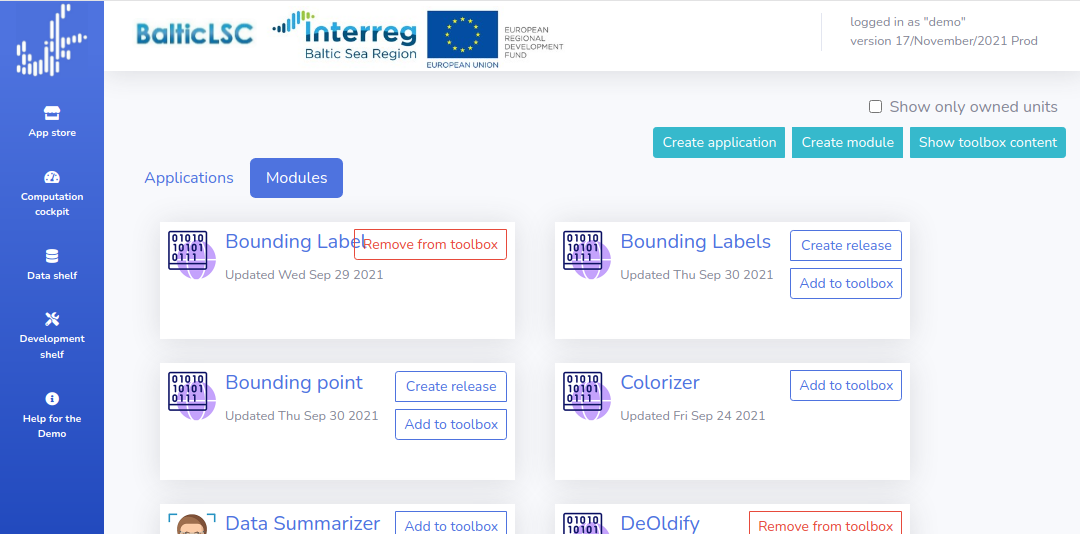
\includegraphics[width=0.95\linewidth]{./images/balticlsc-development-shelf.png}
  \caption{Biblioteka jednostek obliczeniowych platformy
    \BalticLSC{}}\label{rys:balticlsc-development-shelf}
\end{figure}
% \end{noindent}

% \begin{noindent}
\begin{figure}[!ht]
  \centering

  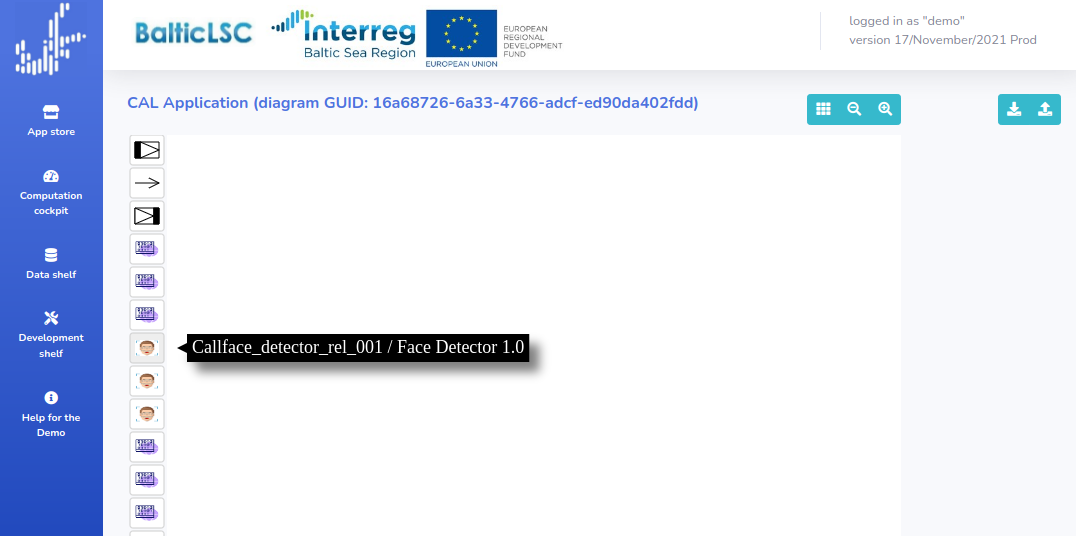
\includegraphics[width=0.95\linewidth]{./images/balticlsc-diagram-toolbox.png}
  \caption{Przybornik dostępny w edytorze diagramów platformy
    \BalticLSC{}}\label{rys:balticlsc-diagram-toolbox}
\end{figure}
% \end{noindent}

% \begin{noindent}
\begin{figure}[!ht]
  \centering

  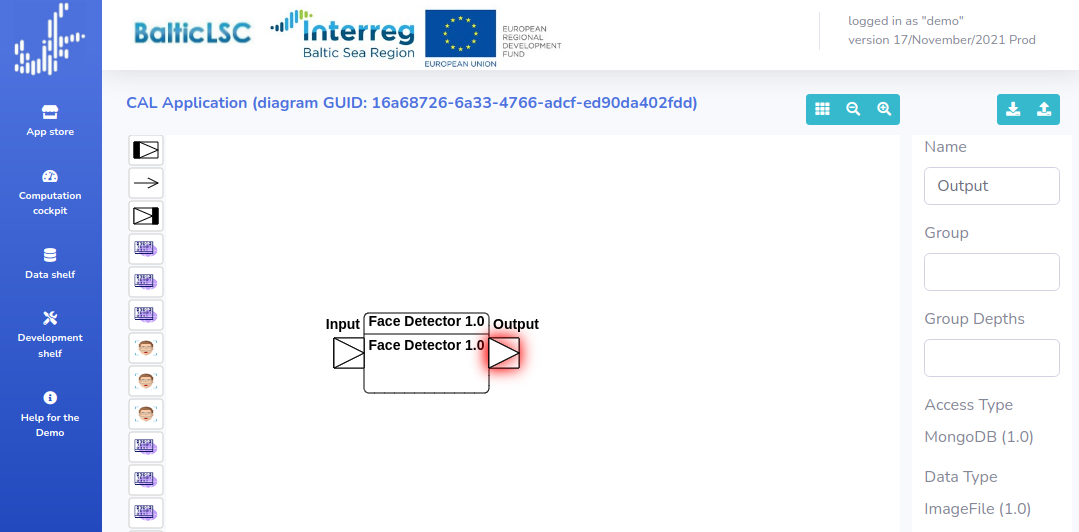
\includegraphics[width=0.95\linewidth]{./images/balticlsc-after-adding-unit-call.png}
  \caption{Edytor diagramów \BalticLSC{} po dodaniu jednostki obliczeniowej z
    przybornika}\label{rys:balticlsc-after-adding-unit-call}
\end{figure}
% \end{noindent}

Rozwiązanie przybornika pozwala użytkownikowi podzielić proces pracy z
jednostkami obliczeniowymi na 2 etapy: wybór interesujących jednostek z listy
potencjalnie
tysięcy dostępnych jednostek obliczeniowych, a później użycie
wybranego podzbioru jednostek na~diagramach.

W edytorze diagramów z \SiriusWeb{} domyślnie nie ma przybornika ani
integracji z~zewnętrznymi serwisami w celu pobrania listy jednostek
obliczeniowych. Definicje wszystkich jednostek obliczeniowych, które mają być
dostępne w modelu muszą być zdefiniowane jako
elementy modelu (\texttt{ComputationUnitRelease}). Mechanizmy dostępne w
metamodelach w formacie \Ecore{} nie pozwalają na komunikację z zewnętrznymi
serwisami,
więc pobieranie danych o~jednostkach obliczeniowych znajdujących się w
przyborniku
danego użytkownika musi zostać zrealizowane na poziomie \SiriusWeb{}.
Ponadto, skoro ma być pobrana zawartość przybornika konkretnego użytkownika,
aplikacja \SiriusWeb{} musi znać jego informacje uwierzytelniające, aby
móc je~dołączyć wysyłając zapytanie \emphgls{API} do serwera \BalticLSC{}.
Szczegóły odtworzenia
mechanizmu przybornika w \SiriusWeb{} oraz jego integracja z
\BalticLSC{} zostały opisane w~kolejnych sekcjach.

\subsection{Pobranie zawartości
	przybornika}\label{sec:pobranie-zawartosci-przybornika}

Serwer aplikacyjny \BalticLSC{} udostępnia interfejs \emphgls{API} w formacie
\emphgls{REST}, który jest używany do komunikacji z aplikacją przeglądarkową
tego
serwisu. Ten interfejs można również wykorzystać w \SiriusWeb{} aby pobrać
zawartość przybornika. W tym celu należy wysłać uwierzytelnione zapytanie
protokołu \emphgls{HTTP} pytając o zasób \texttt{/backend/dev/toolbox/}. W
odpowiedzi zwrócona jest lista składająca się z~informacji o wybranych
jednostkach
obliczeniowych. Zawiera ona wszystkie detale potrzebne do utworzenia obiektu
jednostki obliczeniowej (\texttt{ComputationUnitRelease}) oraz jej wywołania
(\texttt{UnitCall}) w modelu, łącznie z informacjami o zadeklarowanych pinach
tej jednostki.

Należałoby więc z aplikacji przeglądarkowej \SiriusWeb{} wysłać takie
zapytanie do serwera \BalticLSC{}, a następnie wyświetlić otrzymane jednostki
obliczeniowe na ekranie. Już na samym etapie wysyłania zapytania do serwera
\BalticLSC{} pojawiają się dwa problemy.

Pierwszym problemem jest sposób uwierzytelniania użytkownika. Zawartość
przybornika jest powiązana z konkretnym kontem użytkownika w systemie
\BalticLSC{}. Wysyłając więc zapytanie o przybornik należy dodatkowo
załączyć w nagłówku \emphgls{HTTP} \texttt{Authorization}
token uwierzytelniający w formacie \emphgls{JWT}. W tokenie tym znajdują się
informacje o nazwie użytkownika, do którego należy token (pole \texttt{sub}
oraz \texttt{unique\_name}). Zawartość pola z
danymi tokena widoczna jest na listingu~\ref{lst:balticlsc-jwt-payload}.
Ponadto, każdy token \emphgls{JWT} posiada podpis weryfikujący jego
prawdziwość.
Służy on potwierdzeniu, że token został przygotowany przez serwis
\BalticLSC{} w drodze poprawnego logowania do serwisu, a nie został
wytworzony przez osobę próbującą podszyć się pod danego użytkownika.

\begin{lstlisting}[float,
    floatplacement=hb,
    language=java,
    caption={Zawartość pola z danymi w tokenie \emphgls{JWT} z serwisu
      \BalticLSC{}},
    label={lst:balticlsc-jwt-payload}]
{
  "unique_name": "demo",
  "sub": "demo",
  "jti": "bcbbbbe299424a60a3dd4cb918a1364c",
  "sid": "37a970ff48db49e6a5e4c4bb5912d4b4",
  "exp": 1641671342,
  "iss": "wut.balticlsc.eu",
  "aud": "wut.balticlsc.eu"
}
\end{lstlisting}

W pracy magisterskiej założono, że token \emphgls{JWT} zostanie dostarczony do
edytora diagramów z zewnętrznego źródła. W przypadku wykorzystania edytora
diagramów \SiriusWeb{} w innej aplikacji przeglądarkowej, to właśnie ta
zewnętrzna aplikacja przeglądarkowa dostarczy informacje o tokenie
\emphgls{JWT}
podczas wywoływania funkcji rozpoczynającej wyświetlanie diagramu. Zostało to
opisane szczegółowo w sekcji~\ref{sec:uzycie-sirius-web-w-balcitlsc}.

Podczas pracy z pełnym pełnym interfejsem \SiriusWeb{} (a nie tylko samym
edytorem diagramów) został dostarczony przycisk otwierający okno
dialogowe, w którym użytkownik może wprowadzić swój token \emphgls{JWT}.
Znajdują
się w nim także instrukcje jak taki token pozyskać. Ponieważ jest to złożony
proces, który wymaga otworzenia narzędzi programistycznych przeglądarki, został
dostarczony przycisk \emph{\selectlanguage{english}GET DEMO USER TOKEN}, który
pozwala pobrać token użytkownika demonstracyjnego \BalticLSC{}.
Wysyła on zapytanie z prośbą o zalogowanie użytkownika demonstracyjnego,
którego dane logowania są publiczne dostępne, a następnie otrzymany token
uwierzytelniający wprowadza do pola widocznego w oknie dialogowym. W~ten~sposób
można w łatwy sposób otrzymać poprawny token i rozpocząć działanie z
\SiriusWeb{} wykorzystując przybornik użytkownika demonstracyjnego.
Zrzut ekranu przedstawiający okno dialogowe pozwalające wprowadzić token
\emphgls{JWT} użytkownika jest widoczne na
rysunku~\ref{rys:balticlsc-change-jwt-modal}.

% \begin{noindent}
\begin{figure}[!hb]
  \centering

  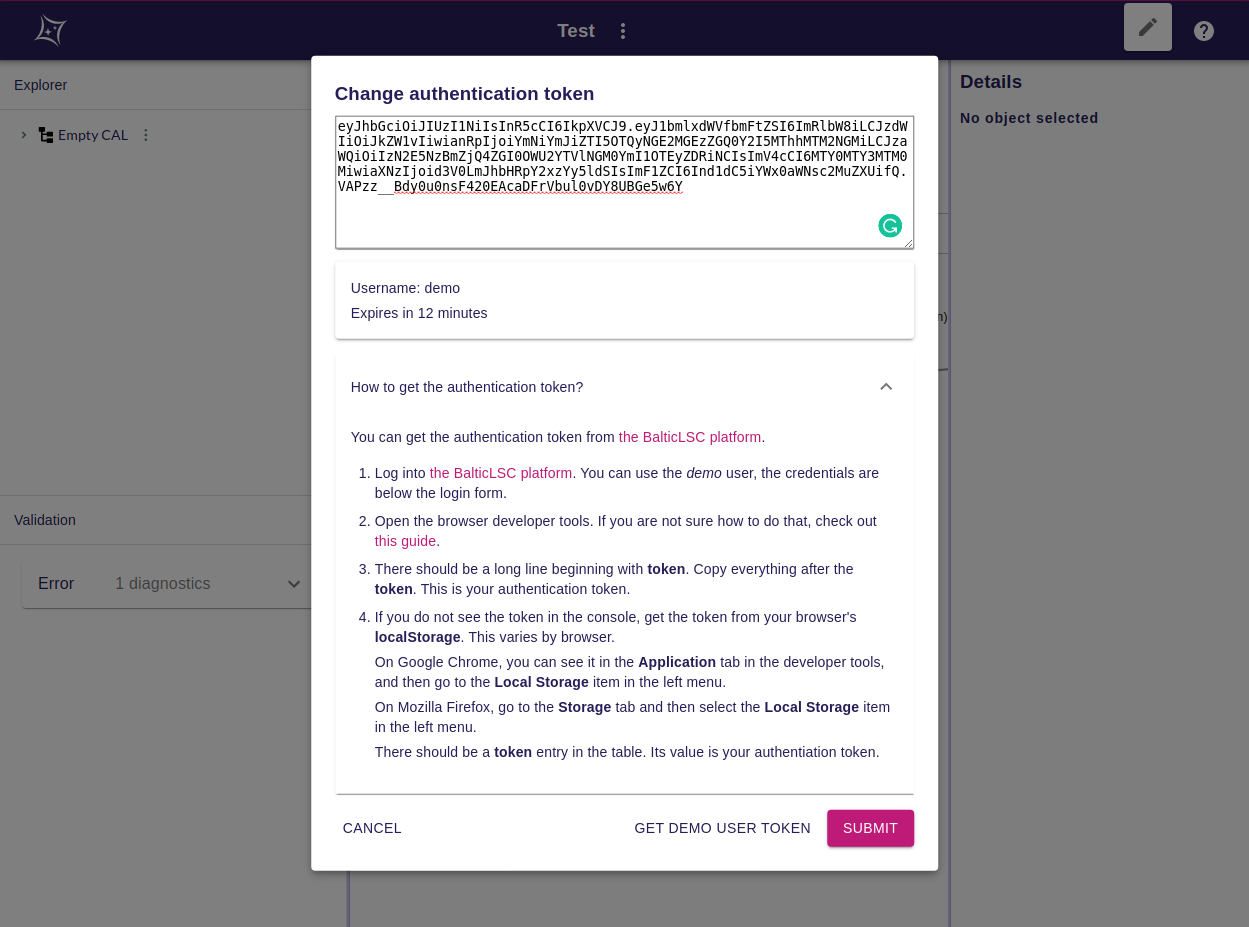
\includegraphics[width=0.95\linewidth]{./images/balticlsc-change-jwt-modal-with-instructions.png}
  \caption{Okno dialogowe do wprowadzenia tokenu \emphgls{JWT}
    użytkownika}\label{rys:balticlsc-change-jwt-modal}
\end{figure}
% \end{noindent}

Drugim z problemów występujących podczas komunikacji z \emphgls{API}
\BalticLSC{} jest mechanizm \emphgls{CORS}~\cite{cors-documentation}. Aktywuje
się on ponieważ serwer
aplikacyjny \BalticLSC{} oraz aplikacja przeglądarkowa \SiriusWeb{} są
uruchomione na różnych adresach w sieci Internet. Odpowiedzi z serwera
aplikacyjnego \BalticLSC{} nie zawierają odpowiednich nagłówków \emphgls{HTTP}
związanych z \emphgls{CORS},
więc przeglądarka blokuje połączenia do tego serwera podczas próby ich wysłania
ze
strony internetowej zawierającej \SiriusWeb{}. W~przypadku edytora
diagramów dostarczonego z \BalticLSC{} \emphgls{CORS} nie występuje, ponieważ
edytor diagramów oraz serwer znajdują się pod tym samym adresem
internetowym\footnote{\url{https://balticlsc.iem.pw.edu.pl/}}, więc
przeglądarka zezwala na te
połączenia bez wymogu dodatkowych nagłówków w odpowiedziach z serwera.

Rozwiązaniem na problem braku nagłówków \emphgls{CORS} w odpowiedziach z
serwera
\BalticLSC{} jest wykorzystanie innego serwera jako pośredniczącego w ruchu
między aplikacją przeglądarkową \SiriusWeb{}, a serwerem \BalticLSC{}
(ang. \emph{\selectlanguage{english}proxy}). Schemat komunikacji między
aplikacją \SiriusWeb{} uruchomioną w przeglądarce a serwerem
\BalticLSC{} z wykorzystaniem serwera pośredniczącego przedstawiono na
rysunku~\ref{rys:balticlsc-proxy-sequence-diagram}.

% \begin{noindent}
\begin{figure}[!hb]
  \centering

  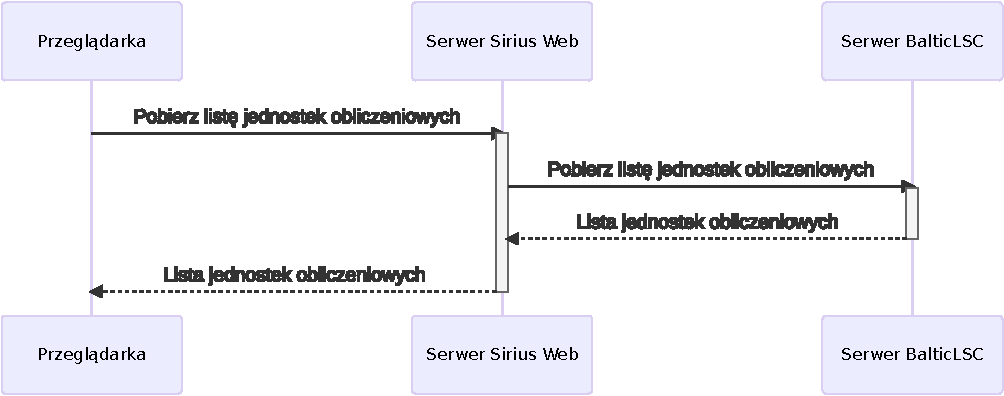
\includegraphics[width=0.95\linewidth]{./images/balticlsc-proxy-sequence-diagram.pdf}
  \caption{Diagram sekwencji pobierania listy jednostek obliczeniowych z
    wykorzystaniem serwera pośredniczącego}\label{rys:balticlsc-proxy-sequence-diagram}
\end{figure}
% \end{noindent}

% Kod źródłowy diagramu (Mermaid)
% https://mermaid-js.github.io/mermaid-live-editor/edit/#eyJjb2RlIjoic2VxdWVuY2VEaWFncmFtXG5wYXJ0aWNpcGFudCBicm93c2VyIGFzIFByemVnbMSFZGFya2FcbnBhcnRpY2lwYW50IHByb3h5IGFzIFNlcndlciBTaXJpdXMgV2ViXG5wYXJ0aWNpcGFudCBiYWx0aWNsc2MgYXMgU2Vyd2VyIEJhbHRpY0xTQ1xuXG5icm93c2VyIC0-PisgcHJveHk6IFBvYmllcnogbGlzdMSZIGplZG5vc3RlayBvYmxpY3plbmlvd3ljaFxucHJveHkgLT4-KyBiYWx0aWNsc2M6IFBvYmllcnogbGlzdMSZIGplZG5vc3RlayBvYmxpY3plbmlvd3ljaFxuXG5iYWx0aWNsc2MgLS0-Pi0gcHJveHk6IExpc3RhIGplZG5vc3RlayBvYmxpY3plbmlvd3ljaFxucHJveHkgLS0-Pi0gYnJvd3NlcjogTGlzdGEgamVkbm9zdGVrIG9ibGljemVuaW93eWNoXG4iLCJtZXJtYWlkIjoie1xuICBcInRoZW1lXCI6IFwiZGVmYXVsdFwiXG59IiwidXBkYXRlRWRpdG9yIjpmYWxzZSwiYXV0b1N5bmMiOnRydWUsInVwZGF0ZURpYWdyYW0iOmZhbHNlfQ
%
% sequenceDiagram
% participant browser as Przeglądarka
% participant proxy as Serwer Sirius Web
% participant balticlsc as Serwer BalticLSC
%
% browser ->>+ proxy: Pobierz listę jednostek obliczeniowych
% proxy ->>+ balticlsc: Pobierz listę jednostek obliczeniowych
%
% balticlsc -->>- proxy: Lista jednostek obliczeniowych
% proxy -->>- browser: Lista jednostek obliczeniowych

Serwerem pośredniczącym może być na przykład serwer aplikacyjny \SiriusWeb{}.
Dodano do niego odpowiedni mechanizm tak, aby wszystkie zapytania
których adres
zaczyna się~od~\texttt{/balticlsc-proxy} przesyłane były do serwera
\BalticLSC{}, a odpowiedzi z serwera zwracane do~oryginalnego nadawcy
zapytania.

W przypadku uruchomienia edytora diagramów \SiriusWeb{} jako część głównej
aplikacji przeglądarkowej \BalticLSC{} pod tym samym adresem co serwer
aplikacyjny tej platformy można zrezygnować z komunikacji z wykorzystaniem
serwera pośredniczącego i wysyłać zapytania bezpośrednio do serwera
aplikacyjnego \BalticLSC{}. W tej sytuacji mechanizm \emphgls{CORS} nie będzie
wykorzystany i przeglądarka pozwoli na wykonanie połączenia.

\subsection{Wyświetlenie zawartości przybornika w Sirius
	Web}\label{sec:wyswietlenie-zawartosci-przybornika-w-sirius-web}

W sekcji~\ref{sec:pobranie-zawartosci-przybornika} opisany został mechanizm, za
pomocą którego aplikacja przeglądarkowa \SiriusWeb{} ma dostęp do listy
jednostek obliczeniowych dodanych do przybornika danego użytkownika. Zawartość
przybornika należy wyświetlić na ekranie w obrębie edytora diagramów, aby
użytkownik mógł z niego skorzystać. Realizacja tej funkcjonalności wymaga
modyfikacji interfejsu użytkownika \SiriusWeb{}.

Warstwa interfejsu użytkownika \SiriusWeb{} napisana jest w języku
\TypeScript{}~\cite{typescript-homepage}, który jest rozszerzeniem języka
\JavaScript{} dodającym
statyczne typowanie zmiennych. Kod~wykorzystuje bibliotekę
\React{}~\cite{react-homepage} do podziału warstwy wizualnej na mniejsze
komponenty i ich wyświetlenie. Podstawowe komponenty, z których można zbudować
edytor modeli bazujący na serwerze aplikacyjnym \SiriusWeb{} są
zlokalizowane i udostępnione w repozytorium \texttt{sirius-components}.
W repozytorium \texttt{sirius-web} są one wykorzystane do zbudowania
przykładowej aplikacji przeglądarkowej do edycji modeli.
Jest ona demonstracją jak można ich użyć i może zostać dostosowana do własnych
potrzeb.

Zdecydowano, że w domyślnym interfejsie użytkownika aplikacji \SiriusWeb{}
zaprezentowanym na rysunku~\ref{rys:sirius-web-base-metamodel-model}
odpowiednie miejsce na wyświetlenie przybornika znajduje się~nad~diagramem,
powyżej paska narzędzi, a poniżej górnej ciemnoniebieskiej belki z tytułem
projektu. Komponent \texttt{Workbench} odpowiedzialny za wyświetlenie edytora
diagramów (całość
interfejsu \SiriusWeb{} oprócz górnej ciemnoniebieskiej belki) nie
ma możliwości pokazania dodatkowych komponentów zdefiniowanych przez
programistę pracującego nad własnym edytorem diagramów. Wyświetla on zawsze
komponenty w ustalonym porządku:

\begin{itemize}
	\item Panel z lewej strony składający się z drzewa elementów projektu na górze oraz informacji diagnostycznych modelu na dole.
	\item Panel główny z edytorem aktualnie wybranego diagramu. Gdy żaden nie jest wybrany, wyświetlone są tam przyciski umożliwiające łatwe stworzenie pierwszego modelu w~projekcie.
	\item Panel z prawej strony składający się z detali aktualnie wybranego elementu diagramu.
\end{itemize}

Chcąc dodać nowy element interfejsu użytkownika wymagane jest skopiowanie kodu
źródłowego komponentu \texttt{Workbench} z repozytorium
\texttt{sirius-components} do własnej kopii repozytorium \texttt{sirius-web} i
skorzystanie w nim bezpośrednio z bardziej podstawowych komponentów.
Nie wszystkie elementy, z których składa się komponent \texttt{Workbench} są
udostępnione do wykorzystania w swoim repozytorium, więc oprócz samego głównego
komponentu należało również skopiować
implementację komponentów odpowiedzialnych za wyświetlenie rozszerzalnych
paneli po lewej i prawej stronie (\texttt{LeftSite}, \texttt{RightSite},
\texttt{Panels}) oraz za~wyświetlenie listy informacji diagnostycznych
(\texttt{ValidationWebSocketContainer}). O~ile~komponenty wizualne związane z
panelami są niezależne od serwera aplikacyjnego \SiriusWeb{}, to komponent
pokazujący
informacje diagnostyczne modelu zawiera w sobie treść subskrypcji WebSocket,
która zależy od interfejsu \emphgls{API} dostarczonego przez serwer. Zmiany w
tym
interfejsie mogą wymagać zmian w kodzie komponentu
\texttt{ValidationWebSocketContainer}. Jednak z uwagi na fakt, że treść tego
komponentu jest skopiowana do własnego repozytorium, komponent ten~może
przestać działać po aktualizacji serwera aplikacyjnego \SiriusWeb{}.
Utrudnia to~utrzymanie aplikacji, ponieważ podczas aktualizacji mogą pojawić
się nieoczekiwane błędy, które widoczne będą dopiero po uruchomieniu aplikacji
przeglądarkowej.

Innym nieudostępnionym z \texttt{sirius-components} komponentem jest
\texttt{OnboardArea}
odpowiedzialny za wyświetlenie przycisków pozwalających na stworzenie nowego
modelu w~projekcie i widoczny jest na
rysunku~\ref{rys:sirius-web-new-model-template}. Jest on pokazywany gdy w
projekcie nie ma jeszcze żadnych
modeli lub nie został wybrany model do wyświetlenia.
Komponent ten jest skomplikowany i zawiera dużo kodu. Jednocześnie w momencie,
gdy jest on wyświetlony, nie ma potrzeby wyświetlać jeszcze przybornika z
\BalticLSC{}. Podjęto decyzję, żeby przed wyborem modelu do wyświetlenia na
diagramie wyświetlić oryginalny komponent \texttt{Workbench}, który wyświetli
komponent \texttt{OnboardArea}. Po wybraniu modelu do wyświetlenia biblioteka
\React{} podmienia komponent widoczny na ekranie na zmodyfikowaną kopię
pochodzącą z lokalnego repozytorium. Dzięki temu zostaje zachowana
funkcjonalność wyświetlenia komponentu \texttt{OnboardArea} bez potrzeby
kopiowania jego implementacji.

Problem związany z nieudostępnieniem wszystkich komponentów bazowych z
% NOTE: allowbreak purposefully terminated with a space (ignore the chktex warning)
\texttt{sirius-\allowbreak components} % chktex 1
jest znany i został zgłoszony autorom
projektu\footnote{
	\url{https://github.com/eclipse-sirius/sirius-components/issues/830}}.
Planują oni również umożliwić dodawanie elementów w panelach po lewej i prawej
stronie\footnote{
	\url{https://github.com/eclipse-sirius/sirius-components/issues/693}}.
Nie ma
natomiast planów umożliwienia dodawania własnych elementów powyżej
wyświetlonego diagramu.

Skopiowane komponenty można dowolnie edytować i rozszerzać. W tym przypadku
zmodyfikowano skopiowany komponent \texttt{Workbench} i dodano w nim
przyciski odpowiedzialne za dodanie wywołania jednostki obliczeniowej do
diagramu. Każdy przycisk zawiera ikonę jednostki, podobnie jak w interfejsie
\BalticLSC{}, a po najechaniu kursorem wyświetla nazwę jednostki oraz jej
wersję, co zostało zaprezentowane na rysunku~\ref{rys:sirius-web-toolbox}.
Ponadto dodany został przycisk
pozwalający na odświeżenie przybornika poprzez ponowne pobranie jego
zawartości.
Do wyświetlenia przycisków zostały wykorzystane komponenty pochodzące
z~biblioteki \emph{Material~UI}~\cite{material-ui-homepage}, która była już
zainstalowana w projekcie \SiriusWeb{}.

\begin{figure}[!ht]
	\centering

	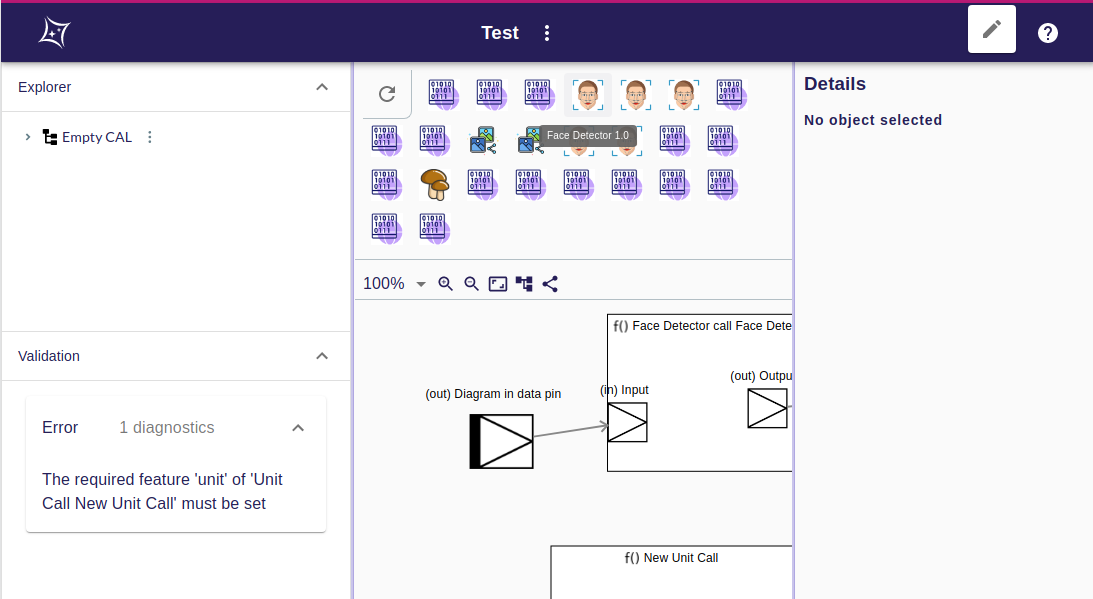
\includegraphics[width=0.95\linewidth]{./images/sirius-web-toolbox.png}
	\caption{Przybornik dodany w
		\SiriusWeb{}}\label{rys:sirius-web-toolbox}
\end{figure}

\subsection{Dodanie wywołania jednostki obliczeniowej do modelu}

W momencie kliknięcia przycisku z ikoną jednostki obliczeniowej do modelu
powinno być~dodane wywołanie tej jednostki (obiekt \texttt{UnitCall}). Jeżeli
jest to pierwszy raz~gdy~wywołanie tej jednostki zostaje dodane do diagramu,
należy przed tym dodać definicję jednostki (obiekt
\texttt{ComputationUnitRelease}) do modelu. Modyfikacja modelu poprzez
aplikację przeglądarkową odbywa się poprzez wysłanie mutacji (\emph{mutation})
w języku \GraphQL{} do serwera aplikacyjnego \SiriusWeb{}, wskazując
przy tym obiekt nadrzędny, do którego ma być dodany obiekt,
oraz szczegóły dodawanego obiektu.

\subsubsection{Wskazywanie miejsca dodania
	obiektu}\label{sec:wskazywanie-miejsca-dodania-elementu}

Aby jednoznacznie określić miejsce, w którym ma być dodany obiekt, należy w
szczegółach mutacji przekazać dwa identyfikatory:

\begin{itemize}
	\item Identyfikator kontekstu edycji danego modelu (\texttt{editingContextId}). Jest to obiekt związany ze szczegółami implementacyjnymi serwera aplikacyjnego \BalticLSC{}. Każdy projekt ma swój kontekst edycji, który można otrzymać wykonując zapytanie \GraphQL{} podając w szczegółach identyfikator projektu.
	\item Identyfikator obiektu nadrzędnego, w którym ma zostać umieszczony nowy obiekt. Model ma strukturę drzewiastą, więc w przypadku tworzenia nowej jednostki obliczeniowej lub~jej~wywołania rodzicem będzie obiekt \texttt{ComputationApplicationRelease}, czyli główny obiekt modelu.
\end{itemize}

Pierwszy z identyfikatorów jest dostępny w komponencie \texttt{Workbench},
który przekazuje go~innym komponentom. Można go przekazać również do
komponentu wyświetlającego przybornik, aby dołączyć go do mutacji dodającej
elementy modelu.

Drugi z identyfikatorów nie jest dostępny w~żadnym z komponentów
znajdujących się~w~skopiowanym repozytorium \texttt{sirius-web}. Komponent
\texttt{ExplorerWebSocketContainer} odpowiedzialny za wyświetlenie drzewa
projektu po lewej stronie interfejsu użytkownika pobiera go podczas
wyświetlania kolejnych poziomów drzewa, jednak nie udostępnia go poza
komponent. Oznacza to, że identyfikator głównego obiektu modelu należy pobrać
inną metodą. Interfejs zapytań \GraphQL{} dostarczony przez \SiriusWeb{} nie
posiada zapytania pozwalającego na pobranie zawartości modelu.

Jednym z możliwych rozwiązań było wykorzystanie tego samego mechanizmu, który
używany jest w komponencie wyświetlającym drzewo projektu, czyli subskrypcji
\GraphQL{} \texttt{treeEvent}. Jest to mechanizm, który pozwala aplikacji
przeglądarkowej na otrzymywanie informacji o zmianach w drzewie modelu na żywo,
tuż po tym jak zostały one wprowadzone. Sprawdza się on dobrze w przypadku
drzewa modelu wyświetlanego ciągle jako część interfejsu użytkownika, ale nie
jest najlepszym rozwiązaniem w przypadku jednorazowego pobierania informacji o
modelu. W tym przypadku mechanizm subskrypcji zostanie wykorzystany tak, jakby
był jednorazowym zapytaniem, ponieważ nasłuchiwanie na zmiany zostanie
zakończone tuż po otrzymaniu odpowiedzi. W porównaniu do zwykłego zapytania
takie rozwiązanie wprowadza dodatkowy narzut w ruchu sieciowym.

Utrudnieniem w pobieraniu identyfikatora głównego obiektu modelu jest fakt, że
subskrypcja \texttt{treeEvent} zwraca informacje jedynie o zawartości tych
obiektów,
których identyfikatory zostały przekazane do subskrypcji. Nawiązuje to do
rozwijania kolejnych poziomów drzewa modelu w interfejsie użytkownika.
Wewnątrz każdego projektu znajduje się sztuczny węzeł reprezentujący dokument
\texttt{Document}, który
w sobie zawiera główny obiekt modelu znany z metamodelu
(\texttt{ComputationApplicationRelease}). Aby
otrzymać identyfikator głównego obiektu modelu należy więc pobrać informacje w
dwóch
krokach: najpierw pobrać informacje o dokumencie, a~później przekazać jego
identyfikator w kolejnej subskrypcji, aby otrzymać identyfikator głównego
obiektu modelu. Diagram sekwencji komunikatów \WebSocket{} wymienianych między
aplikacją przeglądarkową a serwerem w celu otrzymania identyfikatora głównego
obiektu
modelu przedstawiony jest na rysunku~\ref{rys:sirius-web-fetch-model-root-id}.

% Kod źródłowy diagramu:
% https://mermaid-js.github.io/mermaid-live-editor/edit/#eyJjb2RlIjoic2VxdWVuY2VEaWFncmFtXG5wYXJ0aWNpcGFudCBicm93c2VyIGFzIFByemVnbMSFZGFya2FcbnBhcnRpY2lwYW50IGJhY2tlbmQgYXMgU2Vyd2VyIFNpcml1cyBXZWJcblxuYnJvd3NlciAtKSsgYmFja2VuZDogU3RhcnQgdHJlZUV2ZW50IElEIDEgKHB1c3RhIGxpc3RhIHJvendpbmnEmXR5Y2ggd8SZesWCw7N3KVxuYmFja2VuZCAtLSktIGJyb3dzZXI6IE9kcG93aWVkxbogdHJlZUV2ZW50IElEIDEgLSBpZGVudHlmaWthdG9yIGRva3VtZW50dSBtb2RlbHVcbmJyb3dzZXIgLSkrIGJhY2tlbmQ6IFN0b3AgdHJlZUV2ZW50IElEIDFcbmRlYWN0aXZhdGUgYmFja2VuZFxuXG5cbmJyb3dzZXIgLSkrIGJhY2tlbmQ6IFN0YXJ0IHRyZWVFdmVudCBJRCAyIChyb3p3aW5pxJl0eSB3xJl6ZcWCIGRva3VtZW50dSBtb2RlbHUpXG5iYWNrZW5kIC0tKS0gYnJvd3NlcjogT2Rwb3dpZWTFuiB0cmVlRXZlbnQgSUQgMiAtPGJyIC8-IGlkZW50eWZpa2F0b3IgZ8WCw7N3bmVnbyBlbGVtZW50dSBtb2RlbHVcbmJyb3dzZXIgLSkrIGJhY2tlbmQ6IFN0b3AgdHJlZUV2ZW50IElEIDJcbmRlYWN0aXZhdGUgYmFja2VuZCIsIm1lcm1haWQiOiJ7XG4gIFwidGhlbWVcIjogXCJkZWZhdWx0XCJcbn0iLCJ1cGRhdGVFZGl0b3IiOmZhbHNlLCJhdXRvU3luYyI6dHJ1ZSwidXBkYXRlRGlhZ3JhbSI6ZmFsc2V9
% Przekonwertowane do PDF dzięki https://cloudconvert.com/svg-to-pdf (Engine: imagemagick)
%
% sequenceDiagram
% participant browser as Przeglądarka
% participant backend as Serwer Sirius Web
%
% browser -)+ backend: Start treeEvent ID 1 (pusta lista rozwiniętych węzłów)
% backend --)- browser: Odpowiedź treeEvent ID 1 - identyfikator dokumentu modelu
% browser -)+ backend: Stop treeEvent ID 1
% deactivate backend
%
%
% browser -)+ backend: Start treeEvent ID 2 (rozwinięty węzeł dokumentu modelu)
% backend --)- browser: Odpowiedź treeEvent ID 2 -<br /> identyfikator głównego elementu modelu
% browser -)+ backend: Stop treeEvent ID 2
% deactivate backend

% \begin{noindent}
\begin{figure}[!ht]
  \centering

  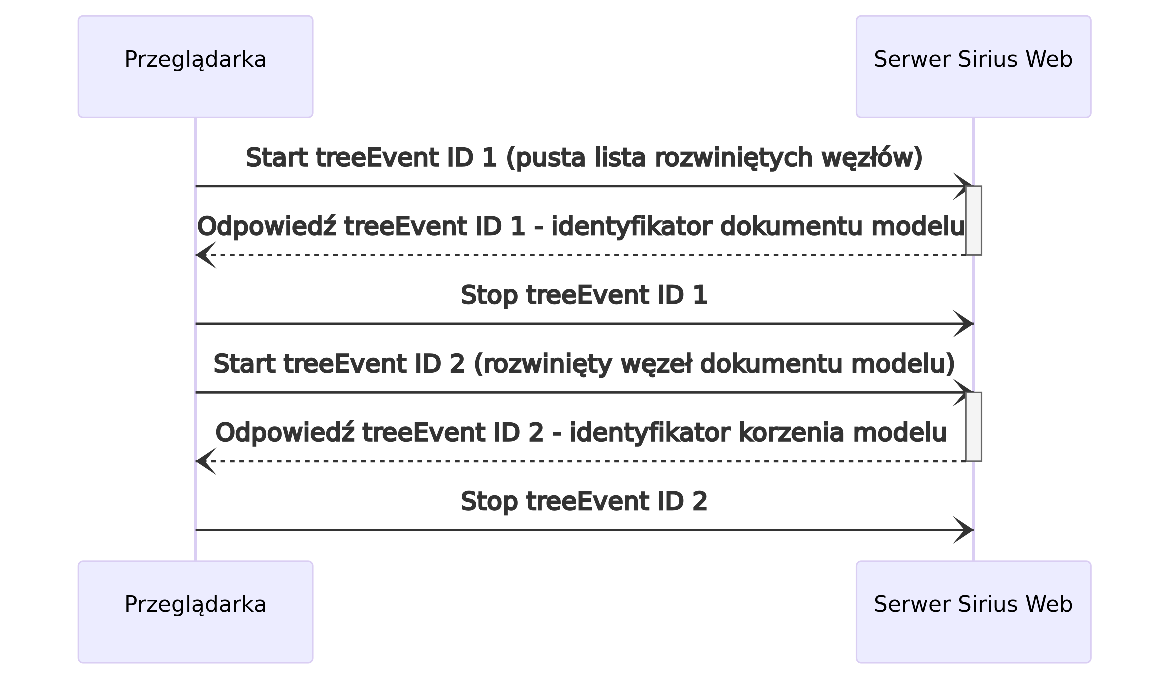
\includegraphics[width=0.90\linewidth]{./images/sirius-web-fetch-model-root-id.pdf}
  \caption{Diagram sekwencji pobierania identyfikatora głównego obiektu
    modelu}\label{rys:sirius-web-fetch-model-root-id}
\end{figure}
% \end{noindent}

\subsubsection{Mutacja dodająca wywołanie jednostki obliczeniowej}

W domyślnym interfejsie użytkownika \SiriusWeb{} obiekty można dodawać na
dwa sposoby: wywołując narzędzia powiązane z metamodelem (opisane w
sekcji~\ref{sec:cal-metamodel-tools}) lub tworząc obiekty bezpośrednio w modelu
zgodnie ze strukturą metamodelu z wykorzystaniem drzewa obiektów.
Ponieważ narzędzia tworzące elementy nie przyjmują parametrów z zewnątrz
dostępna jest~jedynie metoda bezpośredniego tworzenia elementów.

Mutacja
wykorzystywana przez drzewo obiektów modelu to \texttt{createChild}.
W jej parametrach należy przekazać wewnętrzny identyfikator typu obiektu, który
ma
zostać stworzony. Identyfikatory te są tworzone dla każdego obiektu
występującego w
metamodelu w sposób niemożliwy do odgadnięcia, więc otrzymanie informacji o
tych identyfikatorach wymaga wysłania zapytania do serwera.

Tworząc nowe wywołanie jednostki obliczeniowej należy stworzyć wiele obiektów
w~modelu: obiekt \texttt{UnitCall} oraz po jednym obiekcie
\texttt{ComputedDataPin} na każdy pin jednostki obliczeniowej. Jeżeli ta
jednostka
wykorzystywana jest po raz pierwszy w modelu, należy najpierw stworzyć obiekt
\texttt{ComputationApplicationRelease} oraz po jednym obiekcie
\texttt{DeclaredDataPin} na każdy pin jednostki obliczeniowej. Ponadto,
te modyfikacje powinny odbyć się w obrębie jednej transakcji. Z uwagi na
dużą liczbę obiektów do stworzenia w~trybie transakcyjnym, a~także dodatkowe
zapytania sieciowe w celu sprawdzenia czy jednostka była~już~użyta w modelu,
zdecydowano, że zostanie dodana do serwera aplikacyjnego nowa mutacja
\texttt{createUnitCall}, która będzie odpowiedzialna za te operacje.

Dodanie nowej mutacji do serwera \SiriusWeb{} wymagało następujących
kroków:

\begin{itemize}
	\item Dodanie klas typu \emphgls{DTO} w języku \Java{} opisujących strukturę danych wejściowych i wyjściowych mutacji. Klasy oraz ich właściwości muszą mieć odpowiednie adnotacje pochodzące z kodu repozytorium \texttt{sirius-components}, aby~mogły być one przesyłane w języku \GraphQL{}. Dodano klasy i wyliczenia:

	      \begin{itemize}
		      \item \texttt{DataBinding},
		      \item \texttt{Multiplicity},
		      \item \texttt{DeclaredDataPinInput},
		      \item \texttt{ComputationUnitReleaseInput},
		      \item \texttt{CreateUnitCallInput}
		      \item \texttt{CreateUnitCallSuccessPayload}.
	      \end{itemize}

	\item Opisanie dodanych struktur w schemacie danych (\emph{GraphQL
		      schema}).

	\item Implementacja klasy \texttt{MutationCreateUnitCall\-Data\-Fetcher} odpowiedzialnej za~sprawdzenie poprawności danych wejściowych i przekazanie ich do dalszej obsługi.

	\item Implementacja klasy \texttt{CreateUnitCallEventHandler} odpowiedzialnej za odpowiednie zmodyfikowanie modelu.

	      To w tej klasie znajduje się logika sprawdzająca czy jednostka jest już wykorzystywana w~modelu i dodawanie jej definicji jeżeli nie jest użyta lub użycie już dodanej definicji jeżeli istnieje, a później tworzenie wywołania tej jednostki z odpowiednimi wskazaniami na definicję jednostki.

\end{itemize}

Wszystkie dodane klasy zostaną automatycznie wzięte pod uwagę przez serwer
aplikacyjny \SiriusWeb{} podczas obsługi zapytań \emphgls{API} dzięki
mechanizmowi wstrzykiwania zależności (\emph{Dependency Injection}) platformy
\emph{Java Spring}.
W kodzie obsługi mutacji można wykorzystywać klasy języka \Java{} odpowiadające
metaklasom wygenerowane na podstawie metamodelu języka \CAL{} w formacie
\Ecore{}.
Sprawia to, że implementacja jest prostsza i szybsza w porównaniu do
wykonywania tych samych operacji komunikując się przez warstwę zapytań
\GraphQL{}.
Dodatkowo wszystkie zmiany wprowadzane przez kod obsługi mutacji są widoczne
na raz, ponieważ są wykonywane w~obrębie jednej synchronicznej metody. Skutkuje
to atomowością tej~operacji. Przeglądarka nie~dostanie dostanie informacji o
połowicznie zmodyfikowanym modelu --- aktualizacja zostanie przesłana dopiero
po zakończeniu mutacji. Diagram aktywności przedstawiający dodanie wywołania
jednostki obliczeniowej jest przedstawiony
na~rysunku~\ref{rys:sirius-web-create-unit-call-mutation-handler}. Treść
przykładowej mutacji odpowiedzialnej za dodanie jednostki \emph{Bounding
	Labels}
posiadającej dwa piny znajduje się
na~listingu~\ref{lst:sirius-web-createUnitCall-mutation}.

% Źródło:
% https://mermaid-js.github.io/mermaid-live-editor/edit/#eyJjb2RlIjoiZmxvd2NoYXJ0IFREXG4gICAgU3RhcnQoKHh4eCkpXG4gICAgc3R5bGUgU3RhcnQgZmlsbDojMDAwXG4gICAgU3RhcnQgLS0-IFNlYXJjaFVuaXRSZWxlYXNlKFBvc3p1a2FqIG1vZHXFgnUgdyBtb2RlbHUpXG4gICAgU2VhcmNoVW5pdFJlbGVhc2UgLS0-IElmVW5pdFJlbGVhc2VFeGlzdHN7TW9kdcWCIGp1xbw8YnIvPnd5d2_FgmFueTxici8-dyBtb2RlbHU_fVxuXG4gICAgSWZVbml0UmVsZWFzZUV4aXN0cyAtLT58bmllfCBDcmVhdGVDb21wdXRhdGlvblVuaXRSZWxlYXNlKFV0d8Ozcnogb2JpZWt0IENvbXB1dGF0aW9uVW5pdFJlbGVhc2UgaSBkb2RhaiBnbyBkbyBtb2RlbHUpXG4gICAgQ3JlYXRlQ29tcHV0YXRpb25Vbml0UmVsZWFzZSAtLT4gSWZBbGxEZWNsYXJlZERhdGFQaW5zQ3JlYXRlZHtVdHdvcnpvbm88YnIvPndzenlzdGtpZTxici8-emFkZWtsYXJvd2FuZTxici8-cGlueSBtb2R1xYJ1P31cbiAgICBJZkFsbERlY2xhcmVkRGF0YVBpbnNDcmVhdGVkIC0tPnxuaWV8IENyZWF0ZURlY2xhcmVkRGF0YVBpbihVdHfDs3J6IG9iaWVrdCBEZWNsYXJlZERhdGFQaW4gaSBwb3dpxIXFvCB6IENvbXB1dGF0aW9uVW5pdFJlbGVhc2UpXG4gICAgQ3JlYXRlRGVjbGFyZWREYXRhUGluIC0tPiBJZkFsbERlY2xhcmVkRGF0YVBpbnNDcmVhdGVkXG4gICAgSWZBbGxEZWNsYXJlZERhdGFQaW5zQ3JlYXRlZCAtLS0-fHRha3wgQ3JlYXRlVW5pdENhbGxcblxuICAgIElmVW5pdFJlbGVhc2VFeGlzdHMgLS0-fHRha3wgQ3JlYXRlVW5pdENhbGwoVXR3w7NyeiBvYmlla3QgVW5pdENhbGwgaSBkb2RhaiBnbyBkbyBtb2RlbHUpXG4gICAgQ3JlYXRlVW5pdENhbGwgLS0-IElmQWxsQ29tcHV0ZWREYXRhUGluc0NyZWF0ZWR7VXR3b3J6b25vPGJyIC8-d3N6eXN0a2llPGJyIC8-cGlueSBtb2R1xYJ1P31cbiAgICBJZkFsbENvbXB1dGVkRGF0YVBpbnNDcmVhdGVkIC0tPnxuaWV8IENyZWF0ZUNvbXB1dGVkRGF0YVBpbihVdHfDs3J6IG9iaWVrdCBDb21wdXRlZERhdGFQaW4gaSBwb3dpxIXFvCB6IFVuaXRDYWxsKVxuICAgIENyZWF0ZUNvbXB1dGVkRGF0YVBpbiAtLT4gQ29ubmVjdFBpbnMoUG93acSFxbwgQ29tcHV0ZWREYXRhUGluIHogb2Rwb3dpZWRuaW0gRGVjbGFyZWREYXRhUGluKVxuICAgIENvbm5lY3RQaW5zIC0tPiBJZkFsbENvbXB1dGVkRGF0YVBpbnNDcmVhdGVkXG5cbiAgICBJZkFsbENvbXB1dGVkRGF0YVBpbnNDcmVhdGVkIC0tLT58dGFrfCBSZXR1cm5Vbml0Q2FsbChad3LDs8SHIGluZm9ybWFjamUgbyBzdHdvcnpvbnltIFVuaXRDYWxsKVxuICAgIFJldHVyblVuaXRDYWxsIC0tPiBFbmRcbiAgICBFbmQoKFwiIzExMDQ0O1wiKSkiLCJtZXJtYWlkIjoie1xuICBcInRoZW1lXCI6IFwiZGVmYXVsdFwiXG59IiwidXBkYXRlRWRpdG9yIjpmYWxzZSwiYXV0b1N5bmMiOnRydWUsInVwZGF0ZURpYWdyYW0iOmZhbHNlfQ
% Konwertowane do PDF poprzez drukowanie do PDF w Google Chrome.
% Wykorzystanie https://cloudconvert.com/ usuwało tekst z diagramu.
%
% flowchart TD
%     Start((xxx))
%     style Start fill:#000
%     Start --> SearchUnitRelease(Poszukaj jednostki w modelu)
%     SearchUnitRelease --> IfUnitReleaseExists{Jednostka już<br/>wywołana<br/>w modelu?}
%
%     IfUnitReleaseExists -->|nie| CreateComputationUnitRelease(Utwórz obiekt ComputationUnitRelease i dodaj go do modelu)
%     CreateComputationUnitRelease --> IfAllDeclaredDataPinsCreated{Utworzono<br/>wszystkie<br/>zadeklarowane<br/>piny jednostki?}
%     IfAllDeclaredDataPinsCreated -->|nie| CreateDeclaredDataPin(Utwórz obiekt DeclaredDataPin i powiąż z ComputationUnitRelease)
%     CreateDeclaredDataPin --> IfAllDeclaredDataPinsCreated
%     IfAllDeclaredDataPinsCreated --->|tak| CreateUnitCall
%
%     IfUnitReleaseExists -->|tak| CreateUnitCall(Utwórz obiekt UnitCall i dodaj go do modelu)
%     CreateUnitCall --> IfAllComputedDataPinsCreated{Utworzono<br />wszystkie<br />piny jednostki?}
%     IfAllComputedDataPinsCreated -->|nie| CreateComputedDataPin(Utwórz obiekt ComputedDataPin i powiąż z UnitCall)
%     CreateComputedDataPin --> ConnectPins(Powiąż ComputedDataPin z odpowiednim DeclaredDataPin)
%     ConnectPins --> IfAllComputedDataPinsCreated
%
%     IfAllComputedDataPinsCreated --->|tak| ReturnUnitCall(Zwróć informacje o stworzonym UnitCall)
%     ReturnUnitCall --> End
%     End(("#11044;"))

% \begin{noindent}
\begin{figure}[!ht]
  \centering

  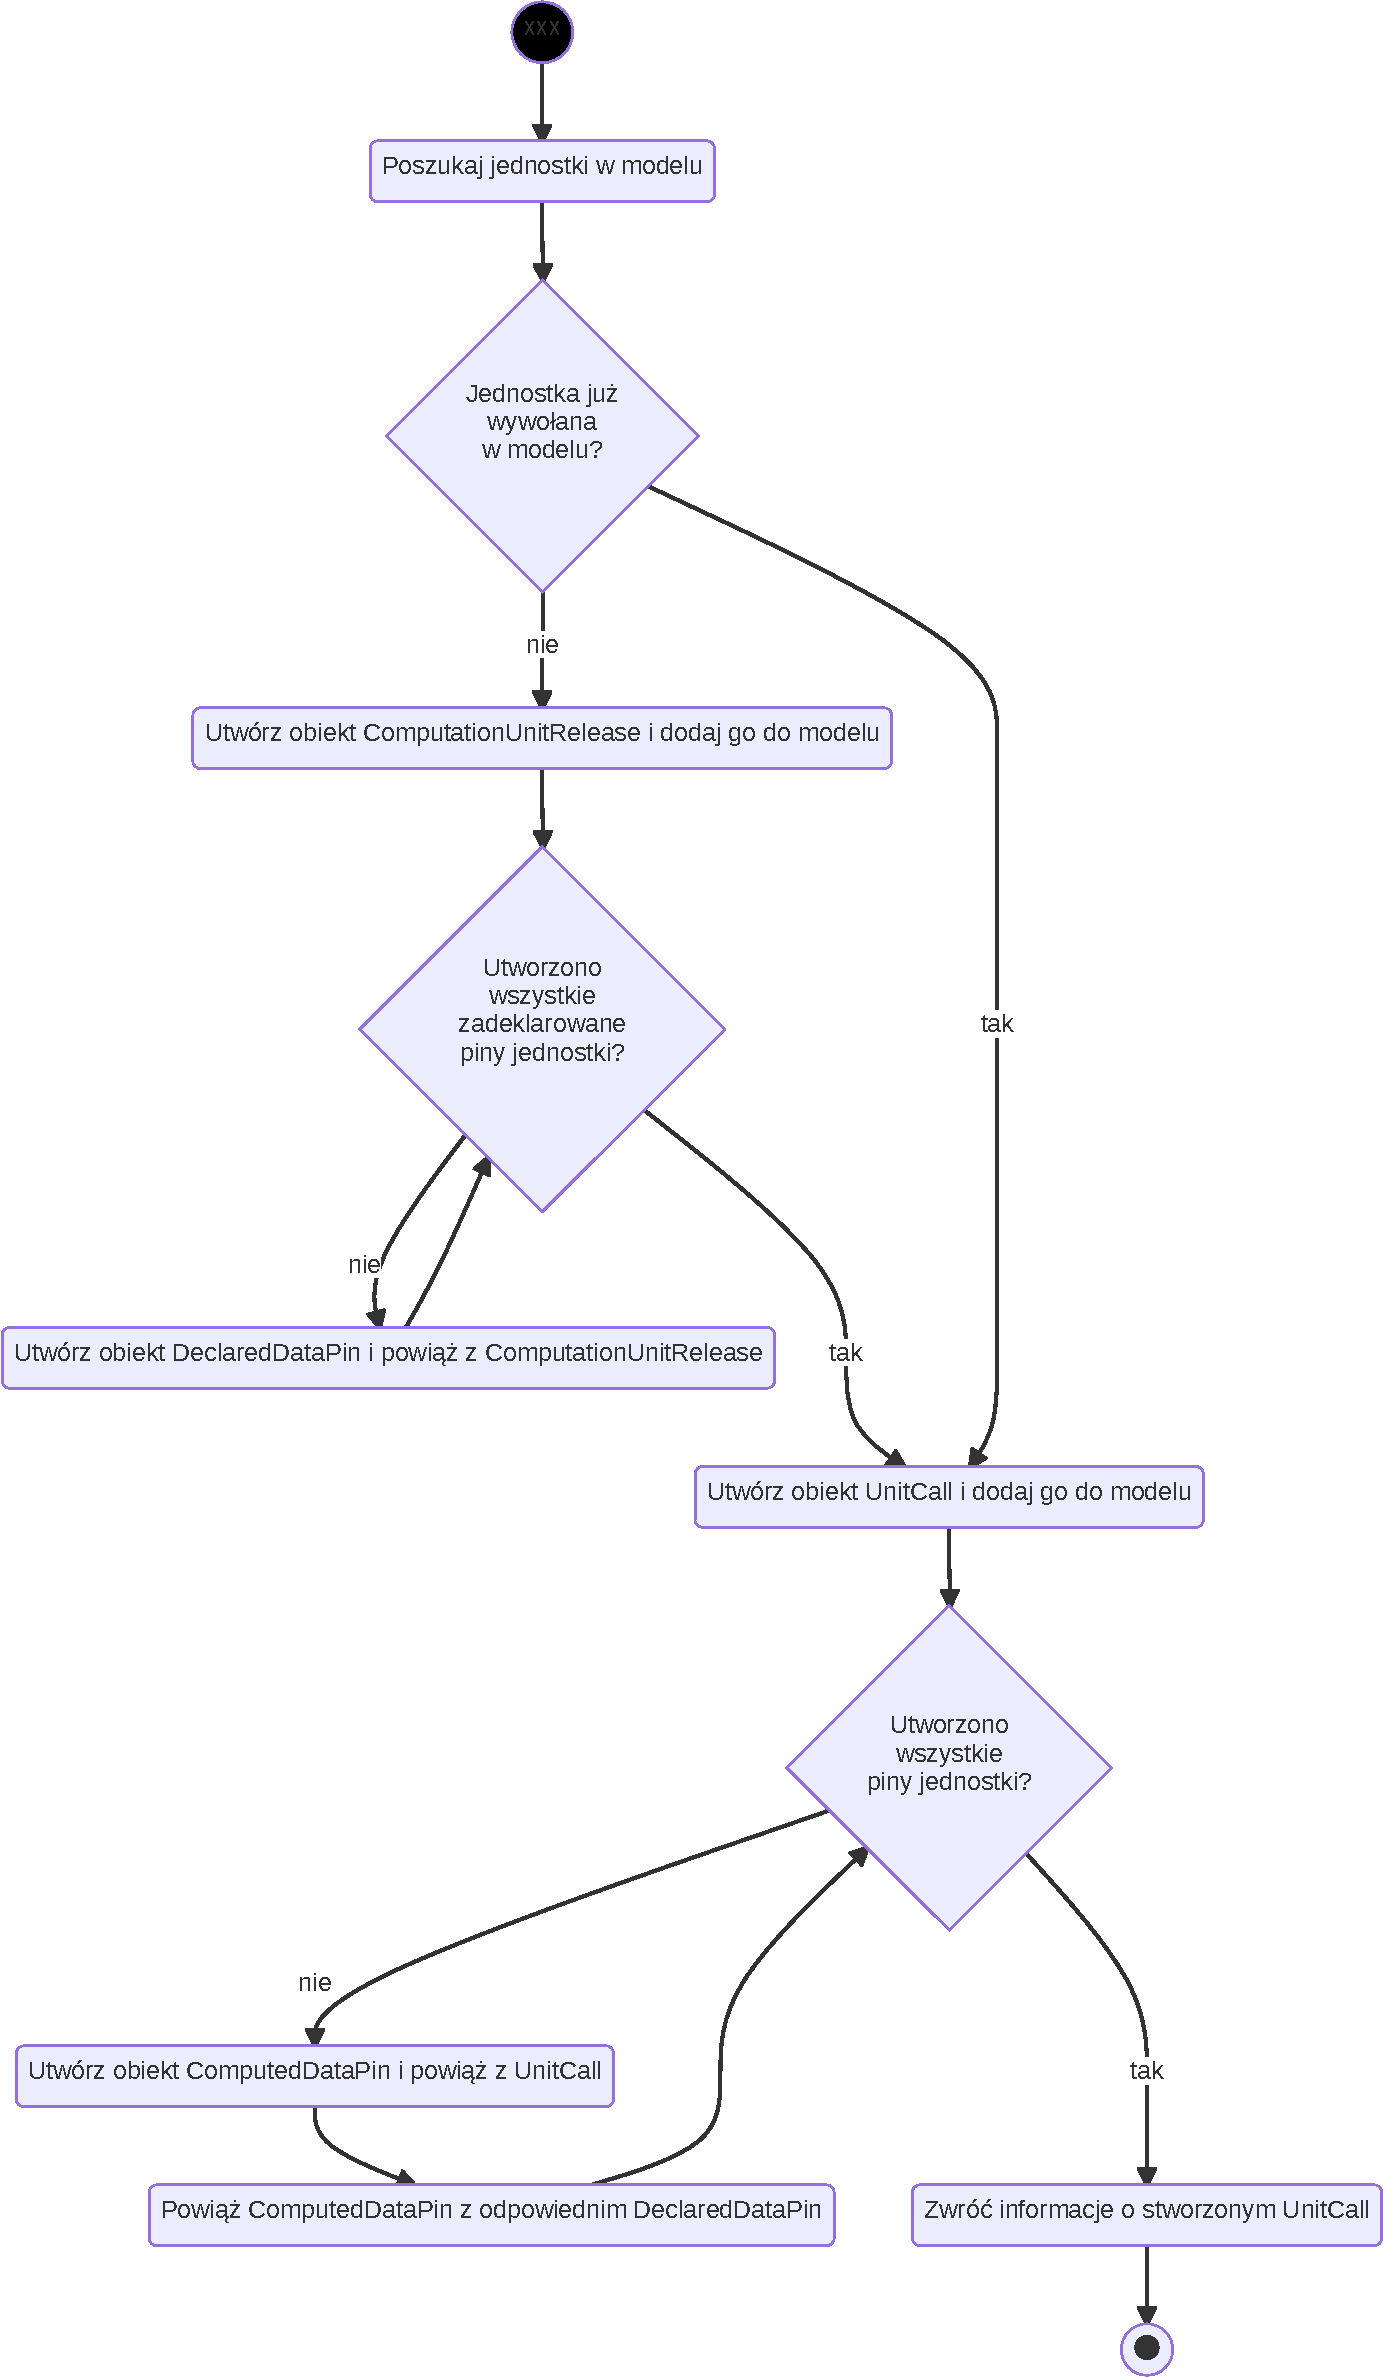
\includegraphics[width=0.70\linewidth]{./images/sirius-web-create-unit-call-mutation-handler.pdf}
  \caption{Diagram aktywności dla dodania nowego wywołania jednostki
    obliczeniowej}\label{rys:sirius-web-create-unit-call-mutation-handler}
\end{figure}
% \end{noindent}

\begin{lstlisting}[float,
    floatplacement=hb,
    % NOTE: graphql is not supported, c adds basic highlighting for strings
    language=c,
    caption={Mutacja \GraphQL{} dodająca wywołanie jednostki obliczeniowej do
      modelu},
    label={lst:sirius-web-createUnitCall-mutation}]
mutation {
  createUnitCall(input: {
    	id: "cfcce8ef-47e3-4f5e-9ecc-847deba46219",
    	rootObjectId:"9e778a79-c5bb-484d-9867-86d4caddec18",
      editingContextId: "a7fdb460-e342-42a6-924e-d31cbb53db69",
      unitRelease: {
        id: "110f65c2-3fc6-411c-9ded-8c8cf96db52d",
        name: "Bounding Labels",
        version: "0.11",
        pins: [
          {
            id: "c915d7a5-dec5-4b60-9fdb-00eed6591cc4",
            name: "Input",
            binding: REQUIRED,
            tokenMultiplicity: SINGLE,
            dataMultiplicity: SINGLE
          },
          {
            id: "76c05ac4-4b34-4053-97e5-8d65748d1485",
            name: "Output",
            binding: PROVIDED,
            tokenMultiplicity: SINGLE,
            dataMultiplicity: SINGLE
          }
        ]
      }
  }) {
    __typename
    ... on CreateUnitCallSuccessPayload {
      id
      createdUnitCall {
        id
        kind
        label
      }
    }
  }
}
\end{lstlisting}

\section{Walidacja semantyczna modelu}\label{sec:walidacja-semantyczna-modelu}

\SiriusDesktop{} posiada funkcjonalność walidacji modelu pod względem
składniowym (na podstawie atrybutów metamodelu) oraz semantycznym (na podstawie
reguł \emph{\selectlanguage{english}Semantic Validation Rule} zdefiniowanych w
pliku \texttt{*.odesign} metamodelu w formacie \Ecore{}), co zostało opisane w
sekcji~\ref{sec:reguly-walidacyjne-metamodel}.

\SiriusWeb{} w swoim interfejsie użytkownika posiada miejsce, w którym
wyświetlają się~pewne informacje diagnostyczne dotyczące modelu. Po każdej
modyfikacji struktury modelu aktualizowane są informacje w dolnej części panelu
po lewej stronie. Zawierają one wyłącznie błędy wynikające z walidacji
składniowej modelu. Pomimo zdefiniowanych reguł walidacji semantycznej, nie są
one wyświetlane w aplikacji przeglądarkowej \SiriusWeb{}. Na
rysunku~\ref{rys:sirius-desktop-and-web-semantic-validation-comparison}
porównano zwracane informacje diagnostyczne w \SiriusWeb{} i \SiriusDesktop{}
dla dwóch modeli o podobnej strukturze. W aplikacji natywnej
widać błędy walidacji semantycznej pochodzące
z~reguł z~metamodelu w formacie \Ecore{}. Błędów tych brakuje w aplikacji
przeglądarkowej. Problem ten~został zgłoszony w repozytorium
\texttt{sirius-web}\footnote{
	\url{https://github.com/eclipse-sirius/sirius-components/issues/816}}.

% \begin{noindent}
\begin{figure}
	\centering
	\begin{subfigure}{.49\textwidth}
		\centering
		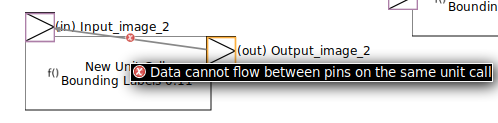
\includegraphics[width=.99\linewidth]{./images/sirius-desktop-example-semantic-validation-rule-failure.png}
		\caption{Błąd walidacji semantycznej w \SiriusDesktop{}}
	\end{subfigure}
	\begin{subfigure}{.49\textwidth}
		\centering
		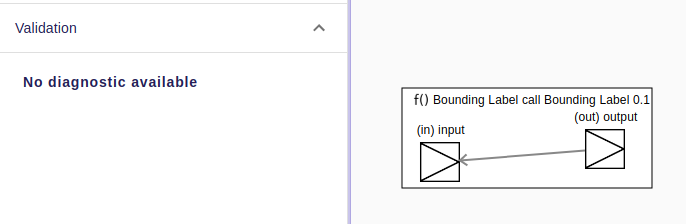
\includegraphics[width=.99\linewidth]{./images/sirius-web-no-emf-semantic-validation.png}
		\caption{Brak błędów walidacji semantycznej w \SiriusWeb{}}
	\end{subfigure}

	\caption{Obsługa reguł walidacji semantycznej z formatu \Ecore{} w \SiriusWeb{}
    i \SiriusDesktop{}}\label{rys:sirius-desktop-and-web-semantic-validation-comparison}
\end{figure}
% \end{noindent}

Oznacza to, że chcąc otrzymać informacje diagnostyczne z walidacji semantycznej
modeli w \SiriusWeb{} należy zaimplementować ten rodzaj walidacji samemu
rozszerzając
serwer aplikacyjny. Informacje z walidacji składniowej modelu są
strumieniowane do przeglądarki za~pomocą subskrypcji \GraphQL{}. Po
wyświetleniu diagramu aplikacja przeglądarkowa rejestruje subskrypcję
\texttt{validationEvent} w interfejsie \emphgls{API} serwera przekazując
identyfikator kontekstu edycji (\texttt{editingContextId}), o którego zmianach
chce być powiadamiana. Po zmianach w~strukturze modelu serwer aplikacyjny
przesyła do przeglądarki wiadomość \texttt{validationEvent} zawierającą listę
informacji diagnostycznych, którą aplikacja przeglądarkowa wyświetla
na~ekranie.

W kodzie źródłowym serwera aplikacyjnego znajduje się klasa
\texttt{Validation\-Description\-Provider}. Jest ona odpowiedzialna za
przygotowanie zestawu funkcji uruchamianych w~momencie, gdy należy sprawdzić
poprawność modelu. Domyślnie korzysta ona z~usługi
\texttt{EMF\-Validation\-Service}, która jest zarejestrowana jako implementacja
interfejsu \texttt{IValidationService}. Dostarcza ona informacji
diagnostycznych z walidacji składniowej modelu. Chcąc dokonać dodatkowo
walidacji
semantycznej należy w metodzie \texttt{getDiagnostics\-Provider} klasy
\texttt{Validation\-Description\-Provider} wykonać tą walidację i~dodać
nowe elementy do listy wynikowych informacji diagnostycznych.

Z uwagi na skomplikowanie dostępu programistycznego do reguł walidacji
semantycznej zdefiniowanych w formacie \Ecore{} zdecydowano, że dodatkowy
mechanizm walidacji semantycznej w \SiriusWeb{} zostanie zaimplementowany
za pomocą osobnych klas języka \Java{}, niekorzystających z reguł
zdefiniowanych
w formacie \Ecore{}. Diagram klas systemu walidacji semantycznej widoczny
jest na rysunku~\ref{rys:sirius-web-semantic-validation-class-diagram}.

% Źródło:
% https://mermaid-js.github.io/mermaid-live-editor/edit/#eyJjb2RlIjoiY2xhc3NEaWFncmFtXG4gICAgZGlyZWN0aW9uIFJMXG4gICAgY2xhc3MgSVNlbWFudGljQ0FMVmFsaWRhdGlvblJ1bGUge1xuICAgICAgICA8PGludGVyZmFjZT4-XG4gICAgICAgIHZhbGlkYXRlKENvbXB1dGF0aW9uQXBwbGljYXRpb25SZWxlYXNlIG1vZGVsKSBMaXN0fkRpYWdub3N0aWN-XG4gICAgfVxuXG4gICAgY2xhc3MgRGF0YUZsb3dEaXJlY3Rpb25cbiAgICBEYXRhRmxvd0RpcmVjdGlvbiAuLnw-IElTZW1hbnRpY0NBTFZhbGlkYXRpb25SdWxlXG4gICAgY2xhc3MgTm9EYXRhRmxvd0N5Y2xlc1xuICAgIE5vRGF0YUZsb3dDeWNsZXMgLi58PiBJU2VtYW50aWNDQUxWYWxpZGF0aW9uUnVsZVxuICAgIGNsYXNzIE5vRGF0YUZsb3dMb29wc1xuICAgIE5vRGF0YUZsb3dMb29wcyAuLnw-IElTZW1hbnRpY0NBTFZhbGlkYXRpb25SdWxlXG5cbiAgICBjbGFzcyBWYWxpZGF0aW9uRGVzY3JpcHRpb25Qcm92aWRlclxuICAgIFZhbGlkYXRpb25EZXNjcmlwdGlvblByb3ZpZGVyIFwiMFwiIC0tPiBcIipcIiBJU2VtYW50aWNDQUxWYWxpZGF0aW9uUnVsZSIsIm1lcm1haWQiOiJ7XG4gIFwidGhlbWVcIjogXCJkZWZhdWx0XCJcbn0iLCJ1cGRhdGVFZGl0b3IiOmZhbHNlLCJhdXRvU3luYyI6dHJ1ZSwidXBkYXRlRGlhZ3JhbSI6ZmFsc2V9
% Przekształcono do PDF za pomocą drukowania SVG do PDF w Google Chrome.
% Potem użyto pdfcrop do przycięcia PDF.
%
% classDiagram
%     direction RL
%     class ISemanticCALValidationRule {
%         <<interface>>
%         validate(ComputationApplicationRelease model) List~Diagnostic~
%     }
%
%     class DataFlowDirection
%     DataFlowDirection ..|> ISemanticCALValidationRule
%     class NoDataFlowCycles
%     NoDataFlowCycles ..|> ISemanticCALValidationRule
%     class NoDataFlowLoops
%     NoDataFlowLoops ..|> ISemanticCALValidationRule
%
%     class ValidationDescriptionProvider
%     ValidationDescriptionProvider --> "0..*" ISemanticCALValidationRule

% \begin{noindent}
\begin{figure}[!hb]
  \centering

  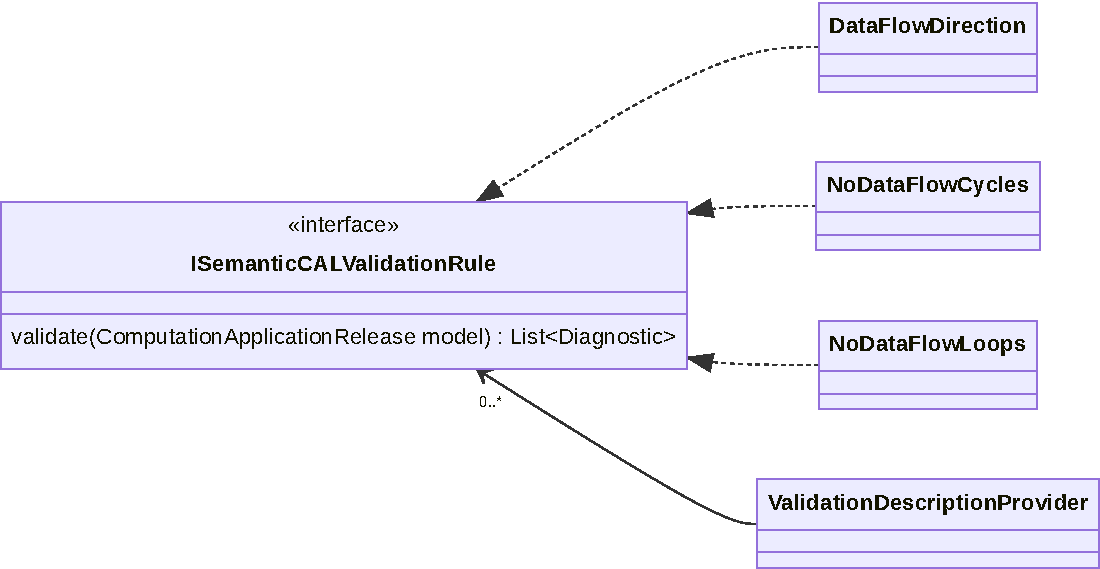
\includegraphics[width=0.95\linewidth]{./images/sirius-web-semantic-validation-class-diagram.pdf}
  \caption{Diagram klas związanych z walidacją semantyczną w
    \SiriusWeb{}}\label{rys:sirius-web-semantic-validation-class-diagram}
\end{figure}
% \end{noindent}

Podstawą architektury do walidacji semantycznej modeli jest interfejs
\texttt{ISemanticCAL\-Validation\-Rule}. Jest on implementowany przez klasy
będące
poszczególnymi regułami walidacji semantycznej modeli języka \CAL{}. Każda
taka reguła musi zaimplementować metodę \texttt{validate}, która otrzymuje
instancję klasy \texttt{ComputationApplicationRelease}. Jest~to klasa
wygenerowana na podstawie metamodelu języka \CAL{} w formacie \Ecore{}
będąca głównym obiektem modelu i~dzięki niej można dotrzeć do dowolnego
elementu modelu. Metoda \texttt{validate} zwraca listę obiektów klasy
\texttt{Diagnostic}
zawierających informacje diagnostyczne o modelu. Jedna reguła walidacji
semantycznej może zwrócić wiele informacji diagnostycznych, ponieważ może
być~naruszona wiele razy przez różne obiekty w modelu. Informacje diagnostyczne
mają różne kategorie --- mogą to być błędy (\emph{error}), ostrzeżenia
(\emph{warning}) lub zwykłe informacje (\emph{info}).

W ramach tej pracy magisterskiej zostały zaimplementowane 3 reguły walidacji
semantycznej w \SiriusWeb{}. Pierwsza z nich (\texttt{DataFlowDirection})
weryfikuje kierunek przepływu
danych na diagramie. Zgłasza ona błąd jeżeli obiekt \texttt{DataFlow} na
diagramie zaczyna się~w~porcie oznaczonym jako wejściowy (\emph{required}) lub
kończy się w porcie oznaczonym jako~wyjściowy (\emph{provided}).

Druga reguła (\texttt{NoDataFlowLoops}) zgłasza jako błędy sytuacje, w których
w modelu występuje
połączenie między pinami na tym samym wywołaniu jednostki obliczeniowej.
Taka jednostka nigdy nie rozpoczęłaby pracy, ponieważ do rozpoczęcia działania
wymaga danych dostarczonych na wszystkich swoich pinach, a więc także danych
dostarczonych od samej siebie, które będą dostępne dopiero po rozpoczęciu
pracy (błędne koło).

Trzecia reguła (\texttt{NoDataFlowCycles}) jest uogólnieniem reguły drugiej.
Wykrywa ona~sytuacje, w których w grafie połączeń \texttt{DataFlow} znajduje
się cykl. Może, ale nie musi to~być~błąd, dlatego informacje diagnostyczne
pochodzące z tej reguły są oznaczone jako ostrzeżenie (\emph{warning}).
Wiadomość
tekstowa zawiera nazwy jednostek obliczeniowych, które wchodzą w skład cyklu.
Reguła ta wykonuje algorytm przeszukiwania grafu w głąb
(\emphgls{DFS})~\cite{wikipedia-dfs}. Po tym następuje próba skrócenia cyklu
poprzez eliminację elementów nieznaczących. Elementem nieznaczącym jest
wierzchołek grafu $x_n$, dla którego istnieje krawędź między  poprzednim
$x_{n-1}$ a kolejnym wierzchołkiem cyklu $x_{n+1}$. Wierzchołek $x_n$ można
usunąć z cyklu. Operacja usuwania nieznaczących elementów jest próbowana dla
wszystkich wierzchołków w cyklu do momentu, gdy nie ma elementów nieznaczących.
Skrócenie cyklu pozwoli użytkownikowi szybciej zlokalizować cykl na diagramie,
ponieważ będzie on zawierał potencjalnie mniej elementów niż ten znaleziony
przez algorytm \emphgls{DFS}. Nie ma gwarancji, że znaleziony cykl po skróceniu
jest najkrótszym cyklem w grafie. Reguła zaprzestaje przeszukiwanie po
znalezieniu pierwszego cyklu.

Za pomocą mechanizmu wstrzykiwania zależności platformy \emph{Java Spring}
wszystkie klasy oznaczone adnotacją \texttt{@Service} implementujące interfejs
\texttt{ISemanticCALValidationRule} są dostępne w klasie
\texttt{ValidationDescriptionProvider}. Wewnątrz implementacji metody
\texttt{getDiagnosticsProvider} jeżeli przetwarzany aktualnie model pochodzi z
metamodelu języka \CAL{} uruchamiane są reguły implementujące interfejs
\texttt{ISemanticCALValidationRule}, a ich wyniki są łączone z wynikami
walidacji składniowej. Implementacja metody zwracającej informacje
diagnostyczne przedstawiona jest na
listingu~\ref{lst:sirius-web-semantic-validation-merge-diagnostics}. Wynikowa
lista informacji diagnostycznych przesyłana
jest do aplikacji przeglądarkowej gdzie jest wyświetlana użytkownikowi. Wyniki
walidacji semantycznej w \SiriusWeb{} widoczne są na
rysunku~\ref{rys:sirius-web-semantic-validation-results}.

\begin{lstlisting}[float,
    floatplacement=hb,
    language=java,
    caption={Metoda zwracająca listę informacji diagnostycznych w \SiriusWeb{}},
    label={lst:sirius-web-semantic-validation-merge-diagnostics}]
private List<Object> getDiagnosticsProvider(VariableManager variableManager) {
    var optionalEditingContext = variableManager.get(IEditingContext.EDITING_CONTEXT, IEditingContext.class);

    var emfDiagnostics = optionalEditingContext.map(this.validationService::validate).orElseGet(List::of);

    var calDiagnostics = optionalEditingContext
            .flatMap(this::extractComputationApplicationRelease)
            .map(applicationRelease ->
                this.validationRules.stream()
                    .flatMap(rule ->
                      rule.validate(applicationRelease).stream()
                    )
                    .collect(Collectors.toList())
            )
            .orElseGet(List::of);

    return Stream.concat(
      emfDiagnostics.stream(),
      calDiagnostics.stream()
    ).collect(Collectors.toList());
}
\end{lstlisting}

% \begin{noindent}
\begin{figure}
	\centering
	\begin{subfigure}{\textwidth}
		\centering
		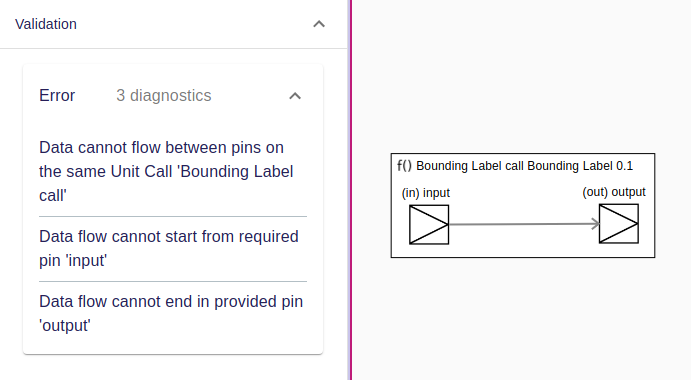
\includegraphics[width=.99\linewidth]{./images/sirius-web-semantic-validation-direction-and-no-loops-rules.png}
		\caption{Błędy walidacji semantycznej związane z kierunkiem połączeń oraz
      pętlami w grafie połączeń}
	\end{subfigure}

  \bigskip

	\begin{subfigure}{\textwidth}
		\centering
		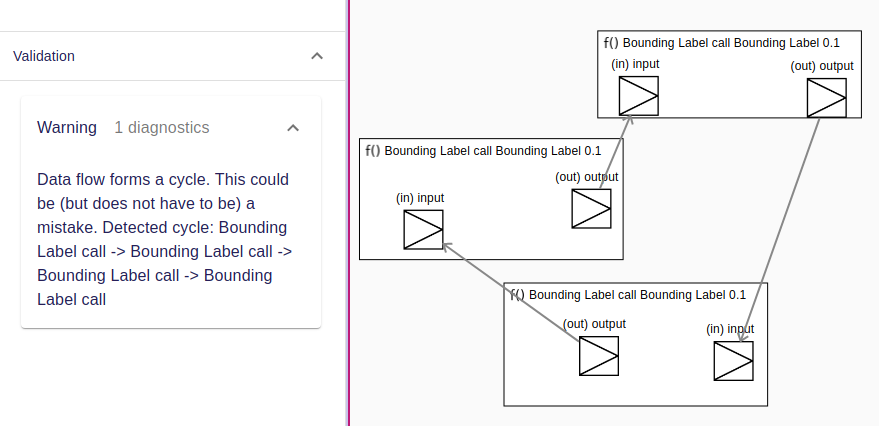
\includegraphics[width=.99\linewidth]{./images/sirius-web-semantic-validation-no-cycles-rule.png}
		\caption{Ostrzeżenie o cyklu w grafie połączeń}
	\end{subfigure}

	\caption{Wyniki dodanego mechanizmu walidacji
  semantycznej}\label{rys:sirius-web-semantic-validation-results}
\end{figure}
% \end{noindent}

Warto zaznaczyć, że aktualizacja informacji diagnostycznych o modelu jest
dokonywana wyłącznie po zmianie struktury modelu (dodaniu, usunięciu elementu,
lub zmianie jego właściwości). Zmiana szczegółów
wizualnych modelu, takich jak zmiana pozycji obiektów na diagramie albo zmiana
ich rozmiaru nie powoduje wywołania kodu odpowiedzialnego za~inspekcję modelu i
zbieranie informacji diagnostycznych. Dzięki temu w momencie zmian wizualnych
diagramu wykonywane jest mniej operacji, co poprawia wydajność edytora.

\section{Użycie edytora Sirius Web w
  BalticLSC}\label{sec:uzycie-sirius-web-w-balcitlsc}

Do tej pory prezentowano edytor modeli \SiriusWeb{} jako osobna aplikacja
przeglądarkowa, niezwiązana z interfejsem użytkownika platformy
\BalticLSC{}. Jedną z możliwości wykorzystania przygotowanego edytora
modeli jest jego integracja jako alternatywny edytor diagramów aplikacji
obliczeniowych w aplikacji przeglądarkowej \BalticLSC{}.
W ramach tej pracy magisterskiej przygotowano kod aplikacji przeglądarkowej
\SiriusWeb{} tak, aby udostępnić osobno sam edytor modeli (komponent
\texttt{Workbench} omówiony w
sekcji~\ref{sec:wyswietlenie-zawartosci-przybornika-w-sirius-web}) w formacie,
który może zostać użyty przez aplikację przeglądarkową \BalticLSC{} w celu
zastąpienia aktualnego edytora diagramów. Przygotowano również
przykładową aplikację w języku \JavaScript{}, która demonstruje wyświetlenie
edytora diagramów z \SiriusWeb{} w części swojego interfejsu.
Integracja \BalticLSC{} i~\SiriusWeb{} pozostaje
poza zakresem pracy magisterskiej.

\subsection{Udostępnienie samodzielnego komponentu edytora diagramów z Sirius
	Web}\label{sec:udostepnienie-samodzielnego-komponentu-Workbench}

Chcąc wyświetlić edytor diagramów z \SiriusWeb{} wewnątrz innej aplikacji
musi być udostępniony interfejs programistyczny \emphgls{API}, który będzie
pozwalał wskazać docelowe miejsce w~aplikacji, w którym ma się
pojawić edytor. Pozostałe elementy aplikacji \SiriusWeb{}, takie
jak~możliwość zarządzania projektami, wybierania projektu do edycji, a także
tworzenia i~usuwania modeli powinny być niedostępne, ponieważ dla lepszych
doświadczeń użytkownika takie operacje powinny być wykonane automatycznie
podczas edycji konkretnej aplikacji obliczeniowej systemu \BalticLSC{}.

Interfejs użytkownika aplikacji \SiriusWeb{} jest napisany w języku
\JavaScript{} z wykorzystaniem biblioteki \React{}~\cite{react-homepage}.
Aplikacja przeglądarkowa \BalticLSC{} jest również napisana w~języku
\JavaScript{}, natomiast korzysta z biblioteki
\emph{Vue.js}~\cite{vue-homepage}.
Z powodu wykorzystania różnych bibliotek kod \SiriusWeb{} musi udostępnić
funkcje zarządzające
wyświetlaniem edytora w języku \JavaScript{}, a nie polegać na mechanizmach
biblioteki \React{} do wyświetlenia komponentu wewnątrz innej aplikacji.

Struktura elementów na stronie internetowej reprezentowana jest jako drzewo
\emphgls{DOM}~\cite{mdn-dom}. Węzły drzewa odpowiadają elementom \emphgls{HTML}
i
za
pomocą różnych metod interfejsu \emphgls{API} drzewa \emphgls{DOM} można
otrzymać do
nich dostęp z poziomu języka \JavaScript{}. Aby wyświetlić komponent biblioteki
\React{} należy znaleźć element drzewa \emphgls{DOM} gdzie komponent ma zostać
umiejscowiony, a później przekazać go wraz z instancją komponentu do~metody
\texttt{render} dostępnej w pakiecie \texttt{react-dom} biblioteki
\React{}. Usunięcie tego komponentu ze strony internetowej realizowane jest
poprzez wywołanie metody \texttt{unmountComponentAtNode} z tego samego pakietu
\texttt{react-dom}. Metoda ta oczekuje jako~parametru elementu drzewa
\emphgls{DOM}, w którym wyświetlony jest komponent.

Aby umożliwić wyświetlenie edytora diagramów (komponentu \texttt{Workbench})
bez względu na bibliotekę wykorzystywaną na stronie internetowej przygotowano
moduł w standardzie \emphgls{ESM}~\cite{nodejs-esm-documentation}, który
udostępnia
niezależne od bibliotek funkcje umożliwiające wyświetlenie i usunięcie edytora
diagramów \SiriusWeb{} w wybranym miejscu na stronie internetowej. Diagram
klas tego modułu został przedstawiony na
rysunku~\ref{rys:sirius-web-library-class-diagram}. Udostępnione funkcje modułu
zostały zgrupowane na diagramie w module \texttt{SiriusWebLibrary} ponieważ
w~diagramach klas \emphgls{UML}
nie ma możliwości wyrażenia pojedynczych funkcji niezwiązanych z żadną
klasą\footnote{\url{https://softwareengineering.stackexchange.com/a/301576}}.
Występujący na diagramie typ \texttt{WorkbenchPropertiesResult} jest typem
\texttt{Either} z biblioteki \texttt{fp-ts}~\cite{fp-ts-github}. Z powodu
reprezentacji jako unia typów w języku TypeScript nie mógł zostać dokładnie
przedstawiony na diagramie UML\@.
Kod modułu znajduje się~w~katalogu \directory{frontend / library}.
Do kompilacji modułu wraz z jego zależnościami zostało wykorzystane narzędzie
\emph{Parcel}~\cite{parcel-homepage}.
Dla wstecznej kompatybilności ze standardem modułów
\emph{CommonJS}~\cite{nodejs-commonjs-documentation} został również wydany
moduł w tym formacie.

% Źródło:
% https://mermaid-js.github.io/mermaid-live-editor/edit/#eyJjb2RlIjoiY2xhc3NEaWFncmFtXG4gICAgZGlyZWN0aW9uIFRCXG4gICAgY2xhc3MgQXBwUHJvcGVydGllcyB7XG4gICAgICAgIDw8aW50ZXJmYWNlPj5cbiAgICAgICAgYXV0aFRva2VuOiBzdHJpbmdcbiAgICB9XG5cbiAgICBjbGFzcyBXb3JrYmVuY2hQcm9wZXJ0aWVzIHtcbiAgICAgICAgPDxpbnRlcmZhY2U-PlxuICAgICAgICBlZGl0aW5nQ29udGV4dElkOiBzdHJpbmdcbiAgICB9XG4gICAgQXBwUHJvcGVydGllcyBvLS0gXCIxXCIgV29ya2JlbmNoUHJvcGVydGllcyA6IHdvcmtiZW5jaFByb3BlcnRpZXNcblxuICAgIGNsYXNzIFJlcHJlc2VudGF0aW9uIHtcbiAgICAgICAgPDxpbnRlcmZhY2U-PlxuICAgICAgICBpZDogc3RyaW5nXG4gICAgICAgIGxhYmVsOiBzdHJpbmdcbiAgICAgICAga2luZDogc3RyaW5nXG4gICAgfVxuICAgIFdvcmtiZW5jaFByb3BlcnRpZXMgby0tIFwiMVwiIFJlcHJlc2VudGF0aW9uIDogcmVwcmVzZW50YXRpb25cblxuICAgIGNsYXNzIEFQSVVSTHNJbnB1dCB7XG4gICAgICAgIDw8aW50ZXJmYWNlPj5cbiAgICAgICAgYmFsdGljTFNDQVBJVVJMOiBzdHJpbmdcbiAgICAgICAgc2lyaXVzV2ViSFRUUEFQSVVSTDogc3RyaW5nXG4gICAgICAgIHNpcml1c1dlYldTQVBJVVJMOiBzdHJpbmdcbiAgICB9XG4gICAgQXBwUHJvcGVydGllcyBvLS0gXCIxXCIgQVBJVVJMc0lucHV0XG5cbiAgICBjbGFzcyBTaXJpdXNXZWJMaWJyYXJ5IHtcbiAgICAgICAgPDxtb2R1bGU-PlxuICAgICAgICByZW5kZXJBcHAoYXBwUHJvcGVydGllczogQXBwUHJvcGVydGllcywgY29udGFpbmVyOiBIVE1MRWxlbWVudCkkICB2b2lkXG4gICAgICAgIHVubW91bnRBcHAoY29udGFpbmVyOiBIVE1MRWxlbWVudCkkIHZvaWRcbiAgICAgICAgcmVzb2x2ZVdvcmtiZW5jaFByb3BlcnRpZXMoKSQgUHJvbWlzZX5Xb3JrYmVuY2hQcm9wZXJ0aWVzUmVzdWx0flxuICAgIH1cblxuICAgICIsIm1lcm1haWQiOiJ7XG4gIFwidGhlbWVcIjogXCJkZWZhdWx0XCJcbn0iLCJ1cGRhdGVFZGl0b3IiOmZhbHNlLCJhdXRvU3luYyI6dHJ1ZSwidXBkYXRlRGlhZ3JhbSI6ZmFsc2V9
% Zmieniono pozycje modułu SiriusWebLibrary na translate(600, 600) w pliku SVG
% SVG -> PDF za pomocą "Print to PDF" z Google Chrome
% Obcięte za pomocą pdfcrop
% classDiagram
%     direction TB
%     class AppProperties {
%         <<interface>>
%         authToken: string
%     }
%
%     class WorkbenchProperties {
%         <<interface>>
%         editingContextId: string
%     }
%     AppProperties o-- "1" WorkbenchProperties : workbenchProperties
%
%     class Representation {
%         <<interface>>
%         id: string
%         label: string
%         kind: string
%     }
%     WorkbenchProperties o-- "1" Representation : representation
%
%     class APIURLsInput {
%         <<interface>>
%         balticLSCAPIURL: string
%         siriusWebHTTPAPIURL: string
%         siriusWebWSAPIURL: string
%     }
%     AppProperties -- "1" APIURLsInput : apiURLs
%
%     class ResolveWorkbenchParamsInput {
%         <<interface>>
%         projectId: string
%         authToken: string
%     }
%     ResolveWorkbenchParamsInput -- "1" APIURLsInput : apiURLs
%
%     class SiriusWebLibrary {
%         <<module>>
%         renderApp(appProperties: AppProperties, container: HTMLElement)$  void
%         unmountApp(container: HTMLElement)$ void
%         resolveWorkbenchProperties(ResolveWorkbenchParamsInput)$ Promise~WorkbenchPropertiesResult~
%     }

% \begin{noindent}
\begin{figure}[!hb]
  \centering

  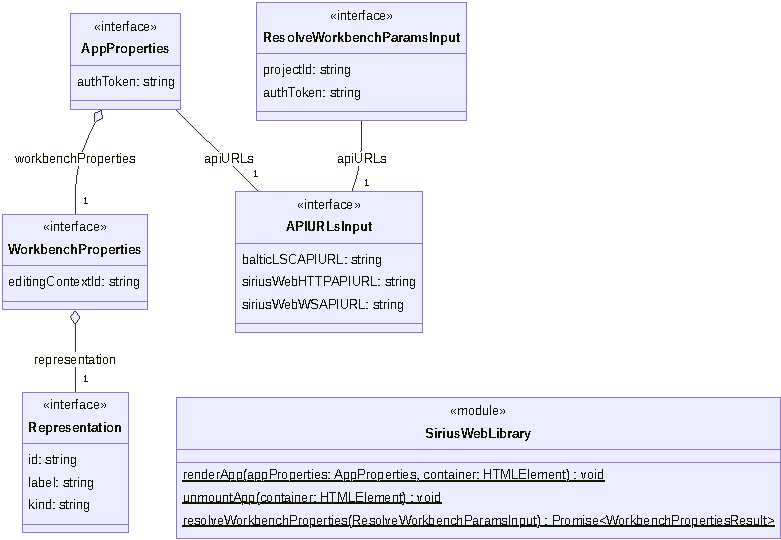
\includegraphics[width=0.99\linewidth]{./images/sirius-web-library-class-diagram.pdf}
  \caption{Diagram klas modułu wyświetlającego edytor diagramów
    \SiriusWeb{}}\label{rys:sirius-web-library-class-diagram}
\end{figure}
% \end{noindent}

Wyświetlenie komponentu \texttt{Workbench} wymaga przekazania mu parametrów
dotyczących modelu, który ma zostać wyświetlony na diagramie. Są to
identyfikator kontekstu edycji \texttt{editingContextId} omówiony w
sekcji~\ref{sec:wskazywanie-miejsca-dodania-elementu} oraz informacje o
reprezentacji modelu do~wyświetlenia. Obie dane są szczegółami
implementacyjnymi aplikacji \SiriusWeb{}. Zakładając, że~w~każdym
projekcie aplikacji \SiriusWeb{} będzie znajdował się wyłącznie jeden
model, który~będzie posiadał jedną reprezentację, informacje te można uzyskać
wysyłając odpowiednie zapytania \GraphQL{} do serwera aplikacyjnego znając
jedynie identyfikator projektu. Aby~uprościć udostępniany
interfejs programistyczny \emphgls{API} modułu stworzono również funkcję
\texttt{resolveWorkbenchProperties}, która oczekuje identyfikatora projektu, a
zwraca parametry potrzebne do wyświetlenia komponentu \texttt{Workbench}, które
uzyskuje poprzez wysłanie zapytań do serwera aplikacyjnego \SiriusWeb{}.
Funkcja ta dodatkowo oczekuje dwóch parametrów:

\begin{itemize}
	\item tokena uwierzytelniającego \emphgls{JWT} aktualnego użytkownika wydanego przez platformę \BalticLSC{} (parametr \texttt{authToken}),
	\item adresów URL serwera aplikacyjnego \BalticLSC{} oraz \SiriusWeb{}
	      (parametr \texttt{apiURLS}).
\end{itemize}

Są one wymagane zarówno do pobrania parametrów edytora diagramów w funkcji
\texttt{resolveWorkbenchProperties}, jak i do późniejszego działania samego
edytora. Diagram sekwencji przedstawiający wykorzystanie udostępnionego modułu
jest widoczny na rysunku~\ref{rys:sirius-web-library-usage-sequence-diagram}.

% Źródło:
% https://mermaid-js.github.io/mermaid-live-editor/edit/#eyJjb2RlIjoic2VxdWVuY2VEaWFncmFtXG4gICAgcGFydGljaXBhbnQgTGliQ29uc3VtZXIgYXMgS29kIHd5a29yenlzdHVqxIVjeSBiaWJsaW90ZWvEmSBTaXJpdXMgV2ViXG4gICAgcGFydGljaXBhbnQgTGlicmFyeSBhcyBCaWJsaW90ZWthIHd5xZt3aWV0bGFqxIVjYSBlZHl0b3JcbiAgICBwYXJ0aWNpcGFudCBTaXJpdXNXZWJCYWNrZW5kIGFzIFNlcndlciBhcGxpa2FjeWpueSBTaXJpdXMgV2ViXG4gICAgcGFydGljaXBhbnQgUmVhY3QgYXMgQmlibGlvdGVrYSBSZWFjdFxuXG4gICAgTGliQ29uc3VtZXIgLT4-KyBMaWJyYXJ5IDogcmVzb2x2ZVdvcmtiZW5jaFByb3BlcnRpZXNcbiAgICBub3RlIG92ZXIgTGliQ29uc3VtZXIsTGlicmFyeTogWmF3aWVyYSBJRCBwcm9qZWt0dSwgdG9rZW4gSldULDxiciAvPmFkcmVzIHNlcndlcmEgU2lyaXVzIFdlYlxuICAgIExpYnJhcnkgLT4-KyBTaXJpdXNXZWJCYWNrZW5kIDogZ2V0UHJvamVjdFF1ZXJ5XG4gICAgbm90ZSBvdmVyIExpYnJhcnksU2lyaXVzV2ViQmFja2VuZCA6IFphcHl0YW5pZSBzaWVjaW93ZSBHcmFwaFFMXG5cbiAgICBTaXJpdXNXZWJCYWNrZW5kIC0tPj4tIExpYnJhcnk6IGVkaXRpbmdDb250ZXh0SWQsIFJlcHJlc2VudGF0aW9uXG5cbiAgICBMaWJyYXJ5IC0tPj4tIExpYkNvbnN1bWVyIDogV29ya2JlbmNoUHJvcGVydGllc1xuXG4gICAgTGliQ29uc3VtZXIgLT4-KyBMaWJyYXJ5IDogcmVuZGVyQXBwXG4gICAgTGlicmFyeSAtPj4rIFJlYWN0IDogcmVuZGVyICh3ecWbd2lldGwga29tcG9uZW50IFdvcmtiZW5jaClcbiAgICBSZWFjdCAtLT4-LSBMaWJyYXJ5IDogV3nFm3dpZXRsb25vIGtvbXBvbmVudCBXb3JrYmVuY2hcbiAgICBMaWJyYXJ5IC0tPj4tIExpYkNvbnN1bWVyIDogV3nFm3dpZXRsb25vIGtvbXBvbmVudCBXb3JrYmVuY2hcblxuICAgIG5vdGUgcmlnaHQgb2YgTGliQ29uc3VtZXIgOiBVxbx5dGtvd25payBtb8W8ZSB0ZXJheiBlZHl0b3dhxIcgZGlhZ3JhbVxuXG4gICAgTGliQ29uc3VtZXIgLT4-KyBMaWJyYXJ5IDogdW5tb3VudEFwcFxuICAgIExpYnJhcnkgLT4-KyBSZWFjdCA6IHVubW91bnRDb21wb25lbnRBdE5vZGVcbiAgICBSZWFjdCAtLT4-LSBMaWJyYXJ5IDogVXN1bmnEmXRvIGtvbXBvbmVudCB6ZSBzdHJvbnkgaW50ZXJuZXRvd2VqXG4gICAgTGlicmFyeSAtLT4-LSBMaWJDb25zdW1lciA6IFVzdW5pxJl0byBrb21wb25lbnQgemUgc3Ryb255IGludGVybmV0b3dlaiIsIm1lcm1haWQiOiJ7XG4gIFwidGhlbWVcIjogXCJkZWZhdWx0XCJcbn0iLCJ1cGRhdGVFZGl0b3IiOmZhbHNlLCJhdXRvU3luYyI6dHJ1ZSwidXBkYXRlRGlhZ3JhbSI6ZmFsc2V9
% SVG -> PDF za pomocą Chrome "Print to PDF", a później pdfcrop
% sequenceDiagram
%     participant LibConsumer as Kod wykorzystujący<br />bibliotekę Sirius Web
%     participant Library as Biblioteka<br />wyświetlająca edytor
%     participant SiriusWebBackend as Serwer aplikacyjny<br/>Sirius Web
%     participant React as Biblioteka React
%
%     LibConsumer ->>+ Library : resolveWorkbenchProperties
%     note over LibConsumer,Library: Zawiera ID projektu, token JWT,<br />adres serwera Sirius Web
%     Library ->>+ SiriusWebBackend : getProjectQuery
%     note over Library,SiriusWebBackend : Zapytanie sieciowe GraphQL
%
%     SiriusWebBackend -->>- Library: editingContextId,<br />Representation
%
%     Library -->>- LibConsumer : WorkbenchProperties
%
%     LibConsumer ->>+ Library : renderApp
%     Library ->>+ React : render (wyświetl komponent Workbench)
%     React -->>- Library : Wyświetlono komponent Workbench
%     Library -->>- LibConsumer : Wyświetlono komponent Workbench
%
%     note right of LibConsumer : Użytkownik może teraz edytować diagram
%
%     LibConsumer ->>+ Library : unmountApp
%     Library ->>+ React : unmountComponentAtNode
%     React -->>- Library : Usunięto komponent<br />ze strony internetowej
%     Library -->>- LibConsumer : Usunięto komponent<br />ze strony internetowej

% \begin{noindent}
\begin{figure}[!hb]
  \centering

  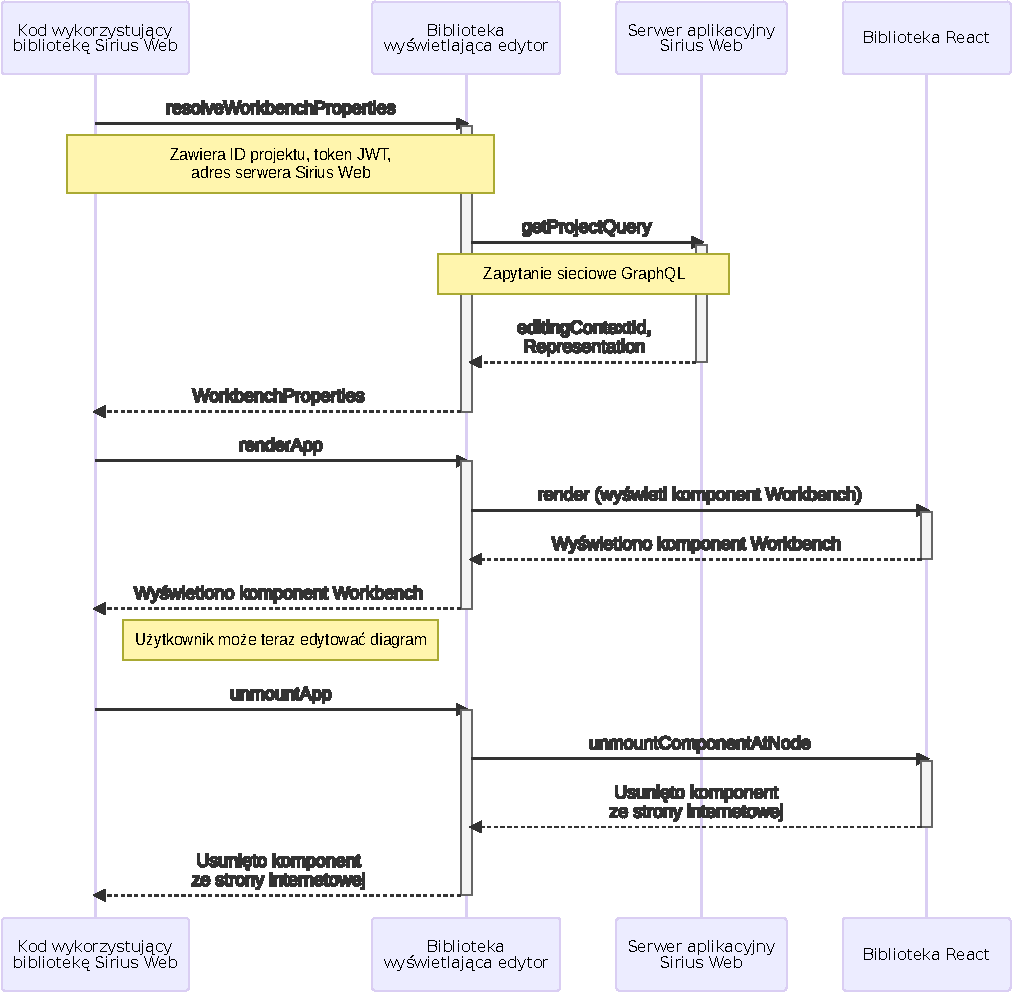
\includegraphics[width=0.95\linewidth]{./images/sirius-web-library-usage-sequence-diagram.pdf}
  \caption{Diagram sekwencji wykorzystania biblioteki wyświetlającej edytor
    diagramów}\label{rys:sirius-web-library-usage-sequence-diagram}
\end{figure}
% \end{noindent}

\subsection{Przykładowa aplikacja wykorzystująca samodzielny edytor
	diagramów}\label{sec:przykladowa-aplikacja-wykorzystujaca-edytor}

Wykorzystując bibliotekę \JavaScript{} wyświetlającą edytor diagramów opisaną w
sekcji~\ref{sec:udostepnienie-samodzielnego-komponentu-Workbench} można
zbudować aplikację przeglądarkową, która ten edytor wyświetli. Taki właśnie
przykład wykonano w ramach tej pracy magisterskiej. Kod źródłowy tej aplikacji
znajduje się w katalogu \directory{frontend-library-example}.

Aplikacja jest
napisana w języku \JavaScript{}. Nie wykorzystuje żadnej znanej biblioteki
(na~przykład \React{} czy \emph{Vue.js}) do~wyświetlenia interfejsu
użytkownika.
Aplikacja zawiera jedynie plik \path{index.html} definiujący strukturę strony
internetowej
oraz \path{app.js} zawierający kod~aplikacji. Interfejs użytkownika po
uruchomieniu aplikacji widoczny jest na
rysunku~\ref{rys:example-app-pre-mount}. Widać na nim informacje o
przeznaczeniu tego przykładu, a także dwa pola tekstowe pozwalające na
wprowadzenie identyfikatora projektu do edycji oraz token \emphgls{JWT}
uwierzytelniający użytkownika w systemie \BalticLSC{}. Pierwszą z tych
informacji można otrzymać z paska adresu pełnej aplikacji \SiriusWeb{} ---
jest to kolejny fragment adresu tuż po fragmencie \texttt{project}. Token
\emphgls{JWT} można uzyskać w okna dialogowego pozwalającego go wprowadzić w
pełnej
aplikacji \SiriusWeb{}. Po uzupełnieniu tych danych można
nacisnąć przycisk \emph{Mount application}, który wyświetli edytor diagramów w
dolnej części strony internetowej. Jest to zaprezentowane na
rysunku~\ref{rys:example-app-mounted}. Można
za jego pomocą dowolnie modyfikować i przeglądać model, podobnie jak w pełnej
wersji aplikacji \SiriusWeb{}. Naciśnięcie przycisku \emph{Unmount
	application} schowa edytor ze strony i wróci ona do stanu początkowego,
jak na rysunku~\ref{rys:example-app-pre-mount}.

% \begin{noindent}
\begin{figure}[!ht]
  \centering

  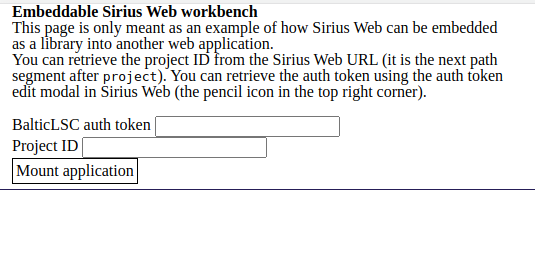
\includegraphics[width=0.95\linewidth]{./images/example-app-pre-mount.png}
  \caption{Przykładowa aplikacja przeglądarkowa przed wyświetleniem
    edytora diagramów}\label{rys:example-app-pre-mount}
\end{figure}
% \end{noindent}

% \begin{noindent}
\begin{figure}[!ht]
  \centering

  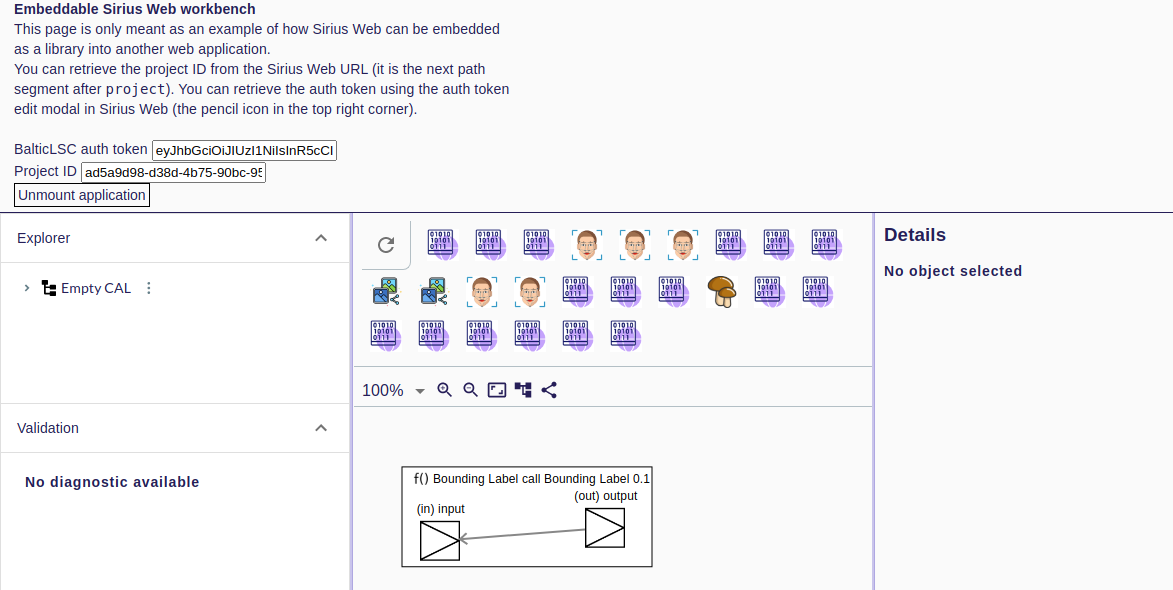
\includegraphics[width=0.95\linewidth]{./images/example-app-mounted.png}
  \caption{Przykładowa aplikacja przeglądarkowa wyświetlająca edytor
    diagramów}\label{rys:example-app-mounted}
\end{figure}
% \end{noindent}

Kod przykładowej aplikacji przeglądarkowej wykonuje operacje w takim samym
porządku jak przedstawiono na diagramie sekwencji na
rysunku~\ref{rys:sirius-web-library-usage-sequence-diagram}. Do uruchomienia
aplikacji używana jest biblioteka \emph{Parcel}. Za jej pomocą można
przygotować również skompilowaną wersję tej~aplikacji, która będzie składała
się z plików \emph{HTML}, \emph{CSS} oraz \JavaScript{}, które będzie można
wyświetlić na
dowolnym serwerze internetowym. Ten przykład pokazuje, że biblioteka
do~wyświetlenia edytora diagramów opisana w
sekcji~\ref{sec:udostepnienie-samodzielnego-komponentu-Workbench} może zostać
wykorzystana w innej aplikacji \JavaScript{} bez wykorzystywania innych
bibliotek.
Do wyświetlenia edytora diagramów potrzebuje jedynie informacji o tokenie
uwierzytelniającym użytkownika oraz identyfikatorze projektu do edycji.
Można będzie tą bibliotekę wykorzystać także w aplikacji przeglądarkowej
platformy \BalticLSC{}.

\subsection{Pomysł integracji Sirius Web i
	BalticLSC}\label{sec:pomysl-integracji-sirius-web-i-balticlsc}

Biblioteka pozwalająca na wyświetlenie edytora diagramów opisana w
sekcji~\ref{sec:udostepnienie-samodzielnego-komponentu-Workbench} może zostać
wykorzystana w dowolnej aplikacji przeglądarkowej, jak pokazano w
sekcji~\ref{sec:przykladowa-aplikacja-wykorzystujaca-edytor}. Oznacza to, że z
pewnymi założeniami można ją również osadzić w interfejsie użytkownika
platformy \BalticLSC{}. Dokonanie tego jest poza zakresem tej pracy
magisterskiej. Poniżej opisano natomiast jak można tego dokonać.

Szczegóły aplikacji obliczeniowych są przechowywane w bazie danych połączonej z
serwerem aplikacyjnym \BalticLSC{}. Serwer aplikacyjny \SiriusWeb{}
oczekuje, że dane edytowanych modeli będą przechowywane w bazie danych w innym
formacie. Oznacza to, że serwery nie mogą korzystać z tej samej bazy danych
jako źródła informacji o aplikacjach obliczeniowych. Serwer \SiriusWeb{}
na czas edytowania danego diagramu będzie posiadał kopię informacji o aplikacji
obliczeniowej, która po zakończeniu edytowania będzie synchronizowana z bazą
danych \BalticLSC{}. To ona będzie źródłem informacji o aplikacjach
obliczeniowych.

Aby zapobiec potrzebie synchronizacji istniejącego modelu \SiriusWeb{} w
momencie rozpoczynania edycji diagramu aplikacji obliczeniowej, model
\SiriusWeb{} może być tworzony na nowo za każdym razem gdy użytkownik
będzie edytował diagram. Model \SiriusWeb{} będzie miał znaczenie tylko
dopóki
użytkownik go edytuje lub przegląda. Gdy użytkownik zamyka edytor diagramów,
po ewentualnym zapisie jego zaktualizowanej zawartości w bazie danych
\BalticLSC{}, model przestaje być używany i może zostać zapomniany.

Diagram komponentów zintegrowanych systemów \SiriusWeb{} oraz
\BalticLSC{} został przedstawiony na
rysunku~\ref{rys:integration-component-diagram}.
Diagram sekwencji przedstawiający ogólną zasadę działania połączonego systemu
jest widoczny na rysunku~\ref{rys:integration-sequence-diagram}.
Działanie rozpoczyna użytkownik chcący wyświetlić zawartość aplikacji
obliczeniowej, zmienić ją, lub stworzyć nową. W tym celu wybiera odpowiedni
przycisk w interfejsie użytkownika \BalticLSC{}.
Po tym przeglądarka wysyła zapytanie do serwera aplikacyjnego \SiriusWeb{}, aby
stworzyć nowy projekt oraz model w nim. Jeżeli jest to
istniejąca aplikacja
obliczeniowa należy odtworzyć jej zawartość w \SiriusWeb{} poprzez dodanie
odpowiednich elementów do nowo stworzonego modelu. Nie istnieje aktualnie żaden
interfejs serwera \SiriusWeb{} pozwalający na dodanie do modelu wielu
elementów na raz, więc jest to
element wymagający rozszerzenia.

% Źródło: source/integration-component-diagram
% https://online.visual-paradigm.com/
% \begin{noindent}
\begin{figure}[!hb]
  \centering

  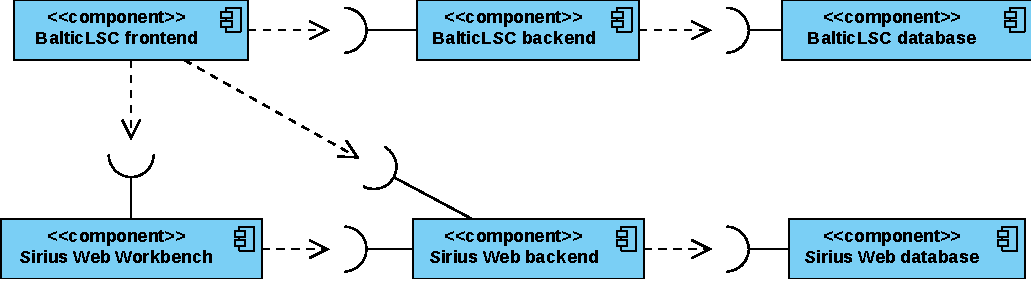
\includegraphics[width=0.95\linewidth]{./images/integration-component-diagram.pdf}
  \caption{Diagram komponentów połączonych systemów \BalticLSC{} i
    \SiriusWeb{}}\label{rys:integration-component-diagram}
\end{figure}
% \end{noindent}

% Źródło:
% https://mermaid-js.github.io/mermaid-live-editor/edit/#eyJjb2RlIjoic2VxdWVuY2VEaWFncmFtXG4gIHBhcnRpY2lwYW50IFVzZXIgYXMgVcW8eXRrb3duaWtcbiAgcGFydGljaXBhbnQgQmFsdGljTFNDVUkgYXMgQXBsaWthY2phIHByemVnbMSFZGFya293YTxiciAvPkJhbHRpY0xTQ1xuICBwYXJ0aWNpcGFudCBCYWx0aWNMU0NCYWNrZW5kIGFzIEFwbGlrYWNqYSBzZXJ3ZXJvd2E8YnIgLz5CYWx0aWNMU0NcbiAgcGFydGljaXBhbnQgQ0FMV2ViQmFja2VuZCBhcyBBcGxpa2FjamEgc2Vyd2Vyb3dhPGJyLz5TaXJpdXMgV2ViXG4gIHBhcnRpY2lwYW50IENBTFdlYlVJIGFzIEJpYmxpb3Rla2EgeiBlZHl0b3JlbTxiciAvPmRpYWdyYW3Ds3dcblxuICBVc2VyIC0-PisgQmFsdGljTFNDVUk6IFJvenBvY3puaWogZWR5Y2rEmSBkaWFncmFtdVxuICBCYWx0aWNMU0NVSSAtPj4rIENBTFdlYkJhY2tlbmQ6IFV0d8OzcnogcHJvamVrdFxuICBDQUxXZWJCYWNrZW5kIC0tPj4tIEJhbHRpY0xTQ1VJOiBQcm9qZWt0IHV0d29yem9ueVxuXG4gIGFsdCBFZHljamEgaXN0bmllasSFY2VqIGFwbGlrYWNqaSBvYmxpY3plbmlvd2VqXG4gICAgQmFsdGljTFNDVUkgLT4-KyBDQUxXZWJCYWNrZW5kOiBEb2RhaiB6YXdhcnRvxZvEhyBhcGxpa2Fjamkgb2JsaWN6ZW5pb3dlaiBkbyBtb2RlbHVcbiAgICBDQUxXZWJCYWNrZW5kIC0tPj4tIEJhbHRpY0xTQ1VJOiBEb2Rhbm9cbiAgZW5kXG5cbiAgQmFsdGljTFNDVUkgLT4-KyBDQUxXZWJVSTogV3nFm3dpZXRsIGVkeXRvciBkaWFncmFtw7N3XG4gIENBTFdlYlVJIC0tPj4tIEJhbHRpY0xTQ1VJOiBXecWbd2lldGxvbm8gZWR5dG9yIGRpYWdyYW3Ds3dcbiAgQmFsdGljTFNDVUkgLS0-Pi0gVXNlcjogV3nFm3dpZXRsb25vIGVkeXRvciBkaWFncmFtw7N3XG5cbiAgbG9vcFxuICAgIFVzZXIgLT4-KyBDQUxXZWJVSTogWm1vZHlmaWt1aiBkaWFncmFtXG4gICAgQ0FMV2ViVUkgLS0-Pi0gVXNlcjogWm1vZHlmaWtvd2FuYSB0cmXFm8SHIGRpYWdyYW11IHdyYXogeiBpbmZvcm1hY2phbWkgZGlhZ25vc3R5Y3pueW1pIHogd2FsaWRhY2ppIG1vZGVsdVxuICBlbmRcblxuICBVc2VyIC0-PisgQmFsdGljTFNDVUk6IFphcGlzeiBkaWFncmFtXG4gIEJhbHRpY0xTQ1VJIC0-PisgQ0FMV2ViQmFja2VuZDogUG9iaWVyeiB6YXdhcnRvxZvEhyBtb2RlbHVcbiAgQ0FMV2ViQmFja2VuZCAtLT4-LSBCYWx0aWNMU0NVSTogWmF3YXJ0b8WbxIcgbW9kZWx1XG5cbiAgQmFsdGljTFNDVUkgLT4-KyBCYWx0aWNMU0NCYWNrZW5kOiBaYXBpc3ogemF3YXJ0b8WbxIcgbW9kZWx1XG4gIEJhbHRpY0xTQ0JhY2tlbmQgLS0-Pi0gQmFsdGljTFNDVUk6IFphcGlzYW5vXG5cbiAgQmFsdGljTFNDVUkgLT4-KyBDQUxXZWJVSTogVWtyeWogZWR5dG9yIGRpYWdyYW3Ds3dcbiAgQ0FMV2ViVUkgLS0-Pi0gQmFsdGljTFNDVUk6IFVrcnl0byBlZHl0b3IgZGlhZ3JhbcOzd1xuXG4gIEJhbHRpY0xTQ1VJIC0tPj4tIFVzZXI6IERpYWdyYW0gemFwaXNhbnlcbiIsIm1lcm1haWQiOiJ7XG4gIFwidGhlbWVcIjogXCJkZWZhdWx0XCJcbn0iLCJ1cGRhdGVFZGl0b3IiOmZhbHNlLCJhdXRvU3luYyI6dHJ1ZSwidXBkYXRlRGlhZ3JhbSI6ZmFsc2V9
% SVG -> PDF za pomocą Chrome "Print to PDF", a potem pdfcrop
% sequenceDiagram
%   participant User as Użytkownik
%   participant BalticLSCUI as Aplikacja przeglądarkowa<br />BalticLSC
%   participant BalticLSCBackend as Aplikacja serwerowa<br />BalticLSC
%   participant CALWebBackend as Aplikacja serwerowa<br/>Sirius Web
%   participant CALWebUI as Biblioteka z edytorem<br />diagramów
%
%   User ->>+ BalticLSCUI: Rozpocznij edycję diagramu
%   BalticLSCUI ->>+ CALWebBackend: Utwórz projekt
%   CALWebBackend -->>- BalticLSCUI: Projekt utworzony
%
%   alt Edycja istniejącej aplikacji obliczeniowej
%     BalticLSCUI ->>+ CALWebBackend: Dodaj zawartość aplikacji obliczeniowej do modelu
%     CALWebBackend -->>- BalticLSCUI: Dodano
%   end
%
%   BalticLSCUI ->>+ CALWebUI: Wyświetl edytor diagramów
%   CALWebUI -->>- BalticLSCUI: Wyświetlono edytor diagramów
%   BalticLSCUI -->>- User: Wyświetlono edytor diagramów
%
%   loop
%     User ->>+ CALWebUI: Zmodyfikuj diagram
%     CALWebUI -->>- User: Zmodyfikowana treść diagramu wraz z informacjami diagnostycznymi z walidacji modelu
%   end
%
%   User ->>+ BalticLSCUI: Zapisz diagram
%   BalticLSCUI ->>+ CALWebBackend: Pobierz zawartość modelu
%   CALWebBackend -->>- BalticLSCUI: Zawartość modelu
%
%   BalticLSCUI ->>+ BalticLSCBackend: Zapisz zawartość modelu
%   BalticLSCBackend -->>- BalticLSCUI: Zapisano
%
%   BalticLSCUI ->>+ CALWebUI: Ukryj edytor diagramów
%   CALWebUI -->>- BalticLSCUI: Ukryto edytor diagramów
%
%   BalticLSCUI -->>- User: Diagram zapisany

% \begin{noindent}
\begin{figure}[!ht]
  \centering

  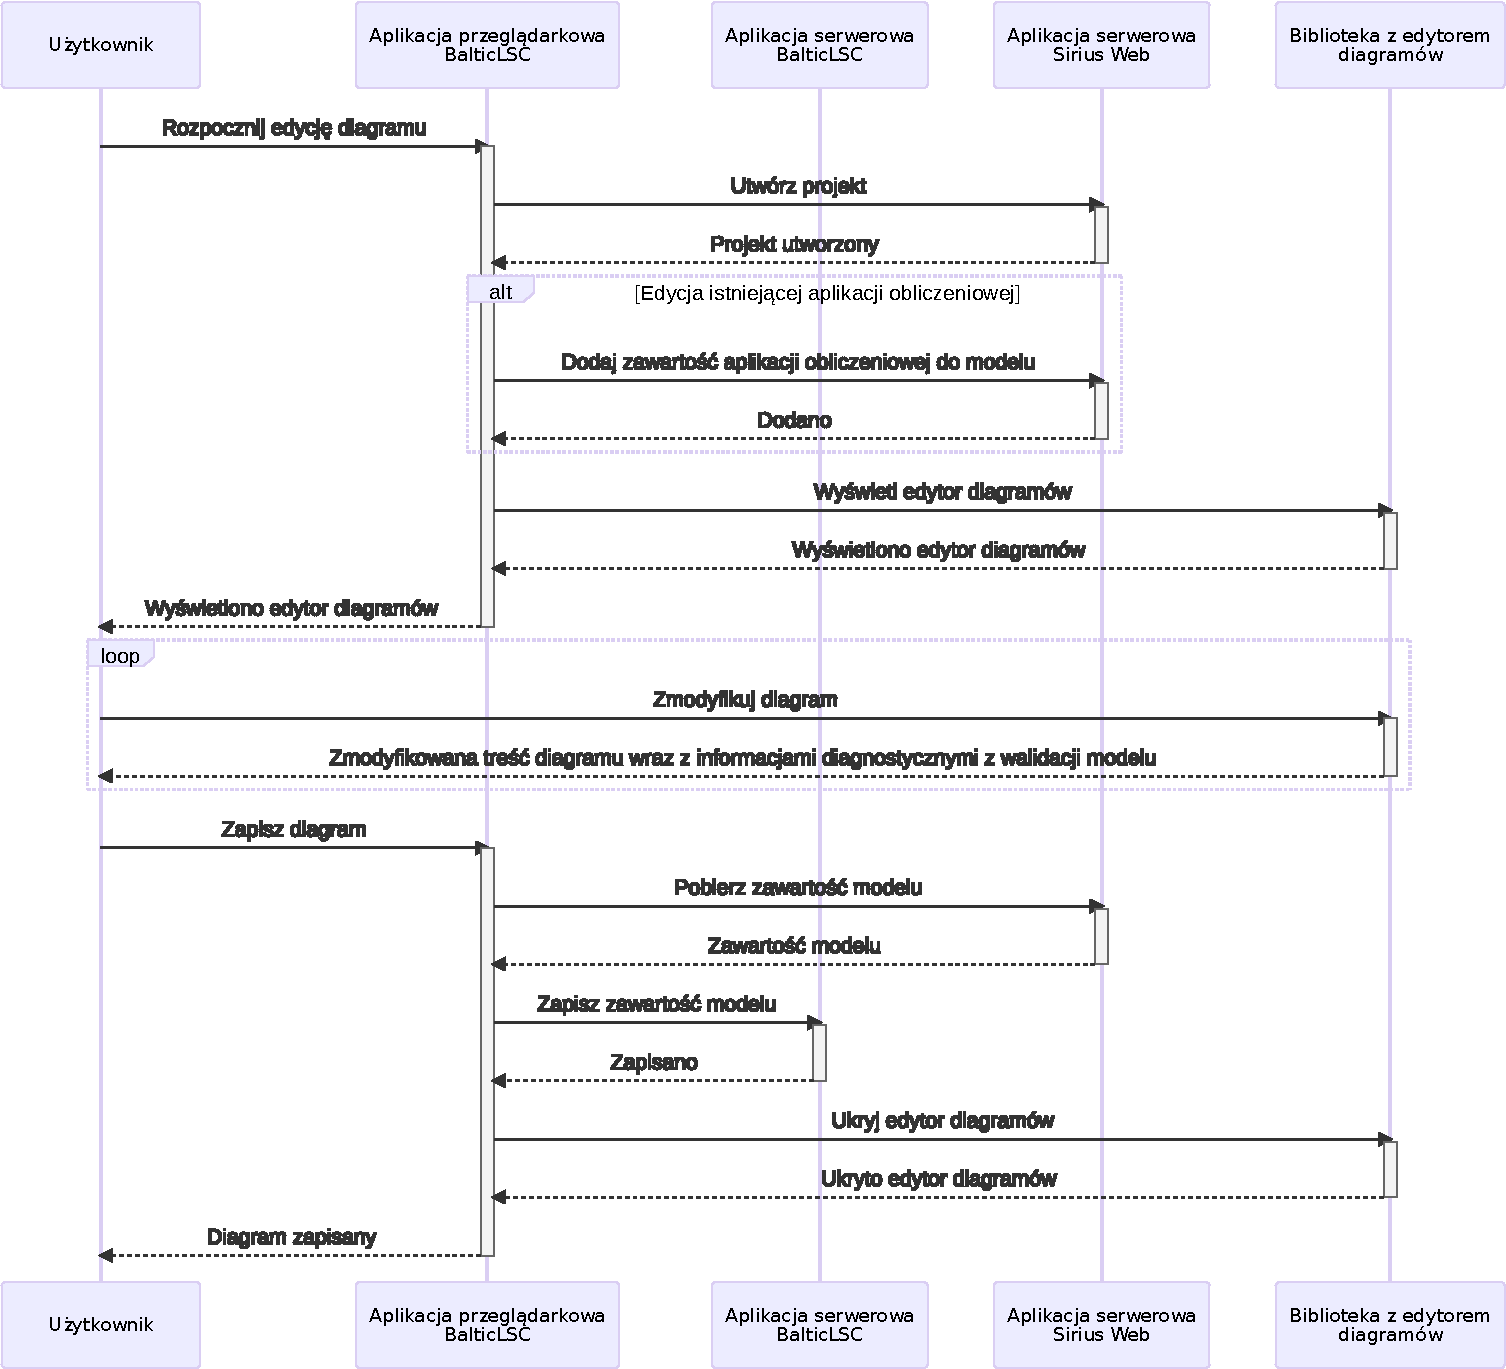
\includegraphics[width=0.99\linewidth]{./images/integration-sequence-diagram.pdf}
  \caption{Diagram sekwencji wykorzystania \SiriusWeb{} w
    \BalticLSC{}}\label{rys:integration-sequence-diagram}
\end{figure}
% \end{noindent}

Po takim przygotowaniu modelu przeglądarka może wyświetlić edytor diagramów
\emph{Sirius~Web} korzystając z przygotowanej biblioteki w języku
\JavaScript{}.
Identyfikator projektu jest znany aplikacji przeglądarkowej \BalticLSC{},
ponieważ został on właśnie przez nią stworzony, a~token uwierzytelniający
\emphgls{JWT} jest również w jej posiadaniu.
Od tego momentu użytkownik może swobodnie przeglądać oraz modyfikować model,
włącznie z wykorzystaniem przybornika omówionego w
sekcji~\ref{sec:integracja-przybornika-balticlsc}. Po każdej zmianie użytkownik
będzie otrzymywał informacje diagnostyczne modelu, także te pochodzące z
walidacji semantycznej poruszonej w
sekcji~\ref{sec:walidacja-semantyczna-modelu}.

Gdy użytkownik będzie chciał zakończyć pracę z diagramem wciśnie on przycisk
odpowiedzialny za zapisanie diagramu. Wtedy aplikacja przeglądarkowa
\BalticLSC{} powinna przesłać zawartość modelu do swojego serwera
aplikacyjnego. Zarówno interfejs \SiriusWeb{} pozwalający na pobranie
zawartości modelu, jak
i interfejs \BalticLSC{} umożliwiający synchronizację zawartości modelu nie
są zaimplementowane i wymagają rozszerzenia.
Po zapisaniu zawartości modelu aplikacja przeglądarkowa \BalticLSC{} może
ukryć edytor modeli wywołując odpowiednią metodą z udostępnionej biblioteki.

Należy zauważyć, że w tej sytuacji w bazie danych \SiriusWeb{} będą
pozostawały przestarzałe modele, z których żaden użytkownik nie skorzysta,
ponieważ za każdym razem tworzony jest nowy projekt. Aby zapobiec
przechowywaniu niepotrzebnych informacji w bazie danych można od czasu do czasu
uruchamiać proces, który czyściłby projekty używane nie później niż~tydzień
przed aktualną datą. W ten sposób w bazie danych pozostawałyby projekty
stworzone najwcześniej tydzień temu, co w znaczny sposób ograniczy ilość
miejsca zajmowanego przez bazę danych.

Jednym z problemów przedstawionego rozwiązania jest możliwość utraty
niezapisanych zmian w modelu podczas przypadkowego wyłączenia przeglądarki lub
przejścia na inną stronę internetową. Informacja o poprzednio utworzonym
projekcie zostałaby zapomniana, a podczas próby edycji aplikacji obliczeniowej
zostałby stworzony nowy model. Aby zapobiec takim sytuacjom aplikacja
przeglądarkowa \BalticLSC{} mogłaby przechowywać listę identyfikatorów
ostatnio edytowanych projektów i umożliwić użytkownikowi powrót do takiego
projektu na~wypadek, gdyby zapomniał on zapisać zmian przed wyjściem z edytora.

Kolejnym z problemów, który może wystąpić, jest zapewnienie kontroli dostępu
do~modeli dla aplikacji obliczeniowych różnych użytkowników systemu
\BalticLSC{}. Na platformie \BalticLSC{} użytkownik może przeglądać
zawartość i edytować jedynie te aplikacje obliczeniowe, które sam stworzył.
Byłoby pożądane, aby podobne zachowanie było przestrzegane w~\SiriusWeb{}.
W ramach tej pracy magisterskiej zaimplementowano mechanizm kontroli dostępu
do~projektów i modeli w \SiriusWeb{} dla zapytań w formacie \emphgls{REST}
oraz
\GraphQL{}. Zapytania dotyczące projektów i modeli wymagają poprawnego
nagłówka \texttt{Authorization}, w którym powinien znajdować się token
uwierzytelniający \emphgls{JWT} pochodzący z aplikacji \BalticLSC{}.
Na~podstawie pola \texttt{sub} zawierającego nazwę użytkownika serwer
aplikacyjny
decyduje o~przyznaniu lub odmowie dostępu do zasobu.

Do pełnej weryfikacji poprawności tokena \emphgls{JWT} brakuje informacji o
sekretnej wartości użytej do stworzenia tego tokena przez \BalticLSC{}. Na
jej podstawie obliczany jest kryptograficzny skrót tokena, który potem może
zostać zweryfikowany (również z wykorzystaniem tej sekretnej wartości) w celu
sprawdzenia prawdziwości tokena. Ujawnienie takiej wartości pozwalałoby na
utożsamienie się z dowolnym użytkownikiem \BalticLSC{}, dlatego w ramach
tej pracy magisterskiej pominięto krok weryfikacji tokenów, aby nie trzeba było
udostępniać sekretnej wartości poza system \BalticLSC{}. W przypadku
integracji systemów należałoby wartość tą~wprowadzić do \SiriusWeb{} w
celu pełnej weryfikacji tokenów \emphgls{JWT}.

O ile zapytania \emphgls{REST} oraz \emph{query} w \GraphQL{} są objęte
kontrolą dostępu, to \emph{subscription} w \GraphQL{} już nie. Dodanie
weryfikacji tokena tam wymaga specjalnej obsługi podczas inicjalizacji
połączenia. Kod ten jest w repozytorium \texttt{sirius-components} i nie został
udostępniony do modyfikacji. Weryfikacja tokenów \emphgls{JWT} nie jest więc
możliwa dla subskrypcji \GraphQL{}. Problem został zgłoszony w repozytorium
\texttt{sirius-components}\footnote{
	\url{https://github.com/eclipse-sirius/sirius-components/issues/846}}.
